%% CUMCM 2025 A 题 论文 — AutoMCM-Pro 流水线产物
%% 编译方式：xelatex main.tex（运行两次以更新交叉引用）

\documentclass[12pt, a4paper]{article}

%% ======================== 宏包导入 ========================
\usepackage{ctex}                    % 中文支持
\usepackage[margin=2.5cm]{geometry}  % 页边距
\usepackage{amsmath, amssymb, amsthm}% 数学公式
\usepackage{graphicx}                % 插图
\usepackage{subcaption}              % 子图
\usepackage{booktabs}                % 三线表
\usepackage{longtable}               % 长表格
\usepackage{array}                   % 表格增强
\usepackage{multirow}                % 跨行单元格
\usepackage{float}                   % 浮动体控制 [H]
\usepackage{hyperref}                % 超链接
\usepackage{enumerate}               % 列表
\usepackage{enumitem}                % 列表定制
\usepackage{listings}                % 代码高亮
\usepackage{xcolor}                  % 颜色
\usepackage{tikz}                    % 流程图
\usepackage{pgfplots}                % 数据可视化
\usepackage{caption}                 % 标题定制
\usepackage{fancyhdr}                % 页眉页脚
\usepackage{setspace}                % 行距
% natbib 与本模板的 plain \bibitem 不兼容（author-year 报错），按 AutoMCM_SOP
% §17 格式合规要求改用标准 \cite/\bibitem，故此处不再加载 natbib
\usepackage{appendix}                % 附录

\pgfplotsset{compat=1.18}
\usetikzlibrary{shapes.geometric, arrows.meta, positioning, calc}

%% ======================== 代码样式 ========================
\definecolor{codegray}{rgb}{0.5,0.5,0.5}
\definecolor{codepurple}{rgb}{0.58,0,0.82}
\definecolor{codeblue}{rgb}{0.13,0.29,0.53}
\definecolor{backcolour}{rgb}{0.97,0.97,0.97}

\lstdefinestyle{pythonstyle}{
    backgroundcolor=\color{backcolour},
    commentstyle=\color{codegray}\itshape,
    keywordstyle=\color{codeblue}\bfseries,
    stringstyle=\color{codepurple},
    basicstyle=\ttfamily\footnotesize,
    breakatwhitespace=false,
    breaklines=true,
    captionpos=b,
    keepspaces=true,
    numbers=left,
    numbersep=5pt,
    numberstyle=\tiny\color{codegray},
    showspaces=false,
    showstringspaces=false,
    showtabs=false,
    tabsize=4,
    frame=single,
    rulecolor=\color{black!20},
    language=Python
}

%% ======================== 页面样式 ========================
% 代码等宽字体改用 DejaVu Sans Mono（含希腊字母 θ 等字形，避免附录代码
% 中 print 语句的 θ 在 lmmono 下缺失）
\setmonofont{DejaVu Sans Mono}[Scale=0.92]

\pagestyle{fancy}
\fancyhf{}
\fancyhead[L]{\small 全国大学生数学建模竞赛}
\fancyhead[R]{\small \leftmark}
\fancyfoot[C]{\thepage}
\renewcommand{\headrulewidth}{0.4pt}

\captionsetup{font=small, labelfont=bf}
\setstretch{1.5}

%% ======================== 自定义命令 ========================
\newtheorem{assumption}{假设}[section]
\newtheorem{definition}{定义}[section]
\newtheorem{theorem}{定理}[section]

\newcommand{\prob}[1]{\mathbf{P}\left(#1\right)}
\newcommand{\E}[1]{\mathbb{E}\left[#1\right]}
\newcommand{\norm}[1]{\left\|#1\right\|}

%% ======================== 文档信息 ========================
\title{
    \vspace{-1cm}
    {\Large \textbf{2025 CUMCM A 题：烟幕干扰弹的投放策略}} \\[0.5em]
    {\large 全国大学生数学建模竞赛参赛论文}
}
\author{}
\date{}

%% ======================== 正文开始 ========================
\begin{document}

\pagenumbering{arabic}
\setcounter{page}{1}

\maketitle
\thispagestyle{plain}

%% ---------------------- 摘要 -------------------------------
\begin{abstract}
\noindent
针对无人机投放烟幕干扰弹掩护真目标对抗空地导弹的作战问题，本文建立了以三维视线遮挡几何为核心的
运动学正演模型，并将投放策略设计归结为连续非线性规划与组合分配两类优化问题，系统地给出了
问题一至问题五的投放策略。
遮蔽判据采用云团中心到"导弹—真目标"视线线段的距离不超过有效半径，多枚烟幕弹的遮蔽时间按
区间并集测度计取；弹道、云团下沉、导弹直线来袭等运动学关系全部按题目给定参数精确建模。
对问题一，按给定策略正演计算得到有效遮蔽时长 $1.410$ s；对问题二，采用物理启发多起点与
坐标轮换精化求解单机单弹优化，将遮蔽时长提升至 $4.611$ s；对问题三，在航向、速度共用的约束下
优化三枚弹的投放时序，得到并集遮蔽 $7.263$ s；对问题四，三架无人机联合投放实现 $15.354$ s；
对问题五，通过"单弹优化—贪心分配—局部精化"的分阶段框架，在 5 架无人机、每机至多 3 枚弹的
约束下对三枚来袭导弹分别形成遮蔽，总遮蔽时长达到 $28.136$ s。灵敏度分析表明，结果对云团
有效半径与导弹速度的依赖在 $10\%$ 扰动下变化不超过约 $10\%$，对真目标参考点高度的建模选择
不敏感，模型整体稳健。全部求解代码经过独立验证脚本核验，关键运动学关系、可行性与并集测度
均通过检查。

\vspace{1em}
\noindent\textbf{关键词：}视线遮挡模型；非线性规划；多起点优化；投放时序调度；多机任务分配
\end{abstract}

\newpage

%% ==================== 1. 问题重述 ====================
\section{问题重述}

烟幕干扰弹通过燃烧或爆炸在目标前方空域形成烟幕云团，遮蔽敌方导弹对真目标的探测，具有
成本低、效费比高的特点。本题以长续航无人机为投放平台：无人机在给定空域巡飞，受领任务后
以 $70\sim 140$ m/s 的速度等高度匀速直线飞行，航向与速度一旦确定不再调整；每架无人机相邻
两枚烟幕干扰弹的投放间隔不少于 $1$ s。烟幕干扰弹脱离无人机后仅在重力作用下运动，起爆后
瞬时形成球状烟幕云团，云团以 $3$ m/s 匀速下沉；云团中心 $10$ m 范围内的烟幕浓度在起爆后
$20$ s 内可为真目标提供有效遮蔽。

来袭武器为三枚空地导弹 M1、M2、M3，飞行速度 $300$ m/s，飞行方向直指为掩护真目标而设置的
假目标（坐标原点）。真目标为半径 $7$ m、高 $10$ m 的圆柱，下底面圆心位于 $(0,200,0)$。
警戒雷达发现导弹时，三枚导弹与五架无人机 FY1$\sim$FY5 的位置均已给定。控制中心立即向
无人机指派任务，需要设计各无人机的飞行方向、飞行速度、烟幕干扰弹投放点与起爆点，使多枚
烟幕干扰弹对真目标的有效遮蔽时间尽可能长，多弹遮蔽时间可以不连续。

需要解决的问题依次为：问题一，FY1 以 $120$ m/s 朝假目标方向飞行、受领任务 $1.5$ s 后投放
$1$ 枚弹、间隔 $3.6$ s 起爆，求对 M1 的有效遮蔽时长；问题二，FY1 单机单弹，优化投放策略使
遮蔽时间最长；问题三，FY1 投放 $3$ 枚弹干扰 M1，给出投放策略并写入 result1.xlsx；问题四，
FY1、FY2、FY3 各投 $1$ 枚弹干扰 M1，结果写入 result2.xlsx；问题五，5 架无人机每架至多投放
$3$ 枚弹，干扰 M1、M2、M3 三枚导弹，结果写入 result3.xlsx。

%% ==================== 2. 问题背景与需要解决的问题 ====================
\section{问题背景与需要解决的问题}

\subsection{问题背景}

烟幕干扰是光电对抗的重要手段，通过在空中形成高浓度烟幕云团衰减来袭武器光电导引头的
探测信号，从而保护己方高价值目标。相比传统的固定式发烟装置，无人机挂载烟幕干扰弹具有
部署灵活、响应迅速、可针对来袭方向定点抛撒等优点，已成为现代战场烟幕干扰的发展方向。
本问题的核心是在已知导弹来袭弹道与无人机布防位置的前提下，通过优化无人机的航迹与弹药
投放时序，在导弹发现真目标之前形成时间上尽量连续、空间上尽量贴合的烟幕遮蔽——本质上是
一个几何运动学约束下的资源调度问题。

\subsection{需要解决的问题}

题目共给出五个递进的问题，遮蔽资源的规模逐级放大。问题一与问题二针对单架无人机单枚弹
的情形：前者在给定投放策略下正演计算对 M1 的有效遮蔽时长，作为模型校准；后者放开航向、
速度、投放点与起爆点的选择，求解单弹最优策略。问题三把弹数放大到三枚，要求 FY1 设计
投放时序与起爆时序，并把结果写入 result1.xlsx。问题四让 FY1、FY2、FY3 三架无人机各投
一枚弹联合干扰 M1，结果写入 result2.xlsx。问题五把规模扩展到 5 架无人机、每架至多 3 枚
弹，对 M1、M2、M3 三枚导弹分别实施干扰，结果写入 result3.xlsx。

作战场景的几何布局如图~\ref{fig:scene3d}~与图~\ref{fig:topview}~所示：三枚导弹从
\texttt{+x} 方向来袭，直指原点处的假目标；五架无人机在导弹来袭方向两侧布防；真目标
位于诱饵正 $y$ 方向 $200$ m 处。

\subsection{数据预处理与场景参数}

题目给定的全部输入均为确定性标量，不存在缺失值与量纲冲突，预处理的重点是把散落在题目
文字中的参数抽取为结构化的场景配置，并做几何层面的核对。抽取后的主要参数如表~
\ref{tab:scenario}~所示，导弹到达假目标的时间与各无人机的航程在建模前先行核算，作为
投放窗口的物理上界；数据预处理阶段同时生成场景三维布局、俯视图与视线几何三张核对图
（图~\ref{fig:scene3d}~、图~\ref{fig:topview}~、图~\ref{fig:los}），供后续建模随时
对照。

\begin{table}[H]
\centering
\caption{场景主要参数（由题目抽取）}
\label{tab:scenario}
\begin{tabular}{lcc}
\toprule
\textbf{参数} & \textbf{数值} & \textbf{用途} \\
\midrule
导弹速度 & $300$ m/s & 视线几何与来袭时刻计算 \\
无人机速度范围 & $[70,\ 140]$ m/s & 优化可行域 \\
云团下沉速度 & $3$ m/s & 云团运动学 \\
云团有效半径 & $10$ m & 遮蔽判据 \\
云团有效时长 & $20$ s & 遮蔽窗口 \\
相邻弹最小投放间隔 & $1$ s & 投放时序约束 \\
真目标参考点 & $(0,200,0)$ & 视线终点 \\
M1/M2/M3 到达假目标时间 & $67.0/63.8/60.4$ s & 投放窗口上界 \\
\bottomrule
\end{tabular}
\end{table}

\begin{figure}[H]
\centering
\begin{minipage}[t]{0.86\textwidth}
\centering
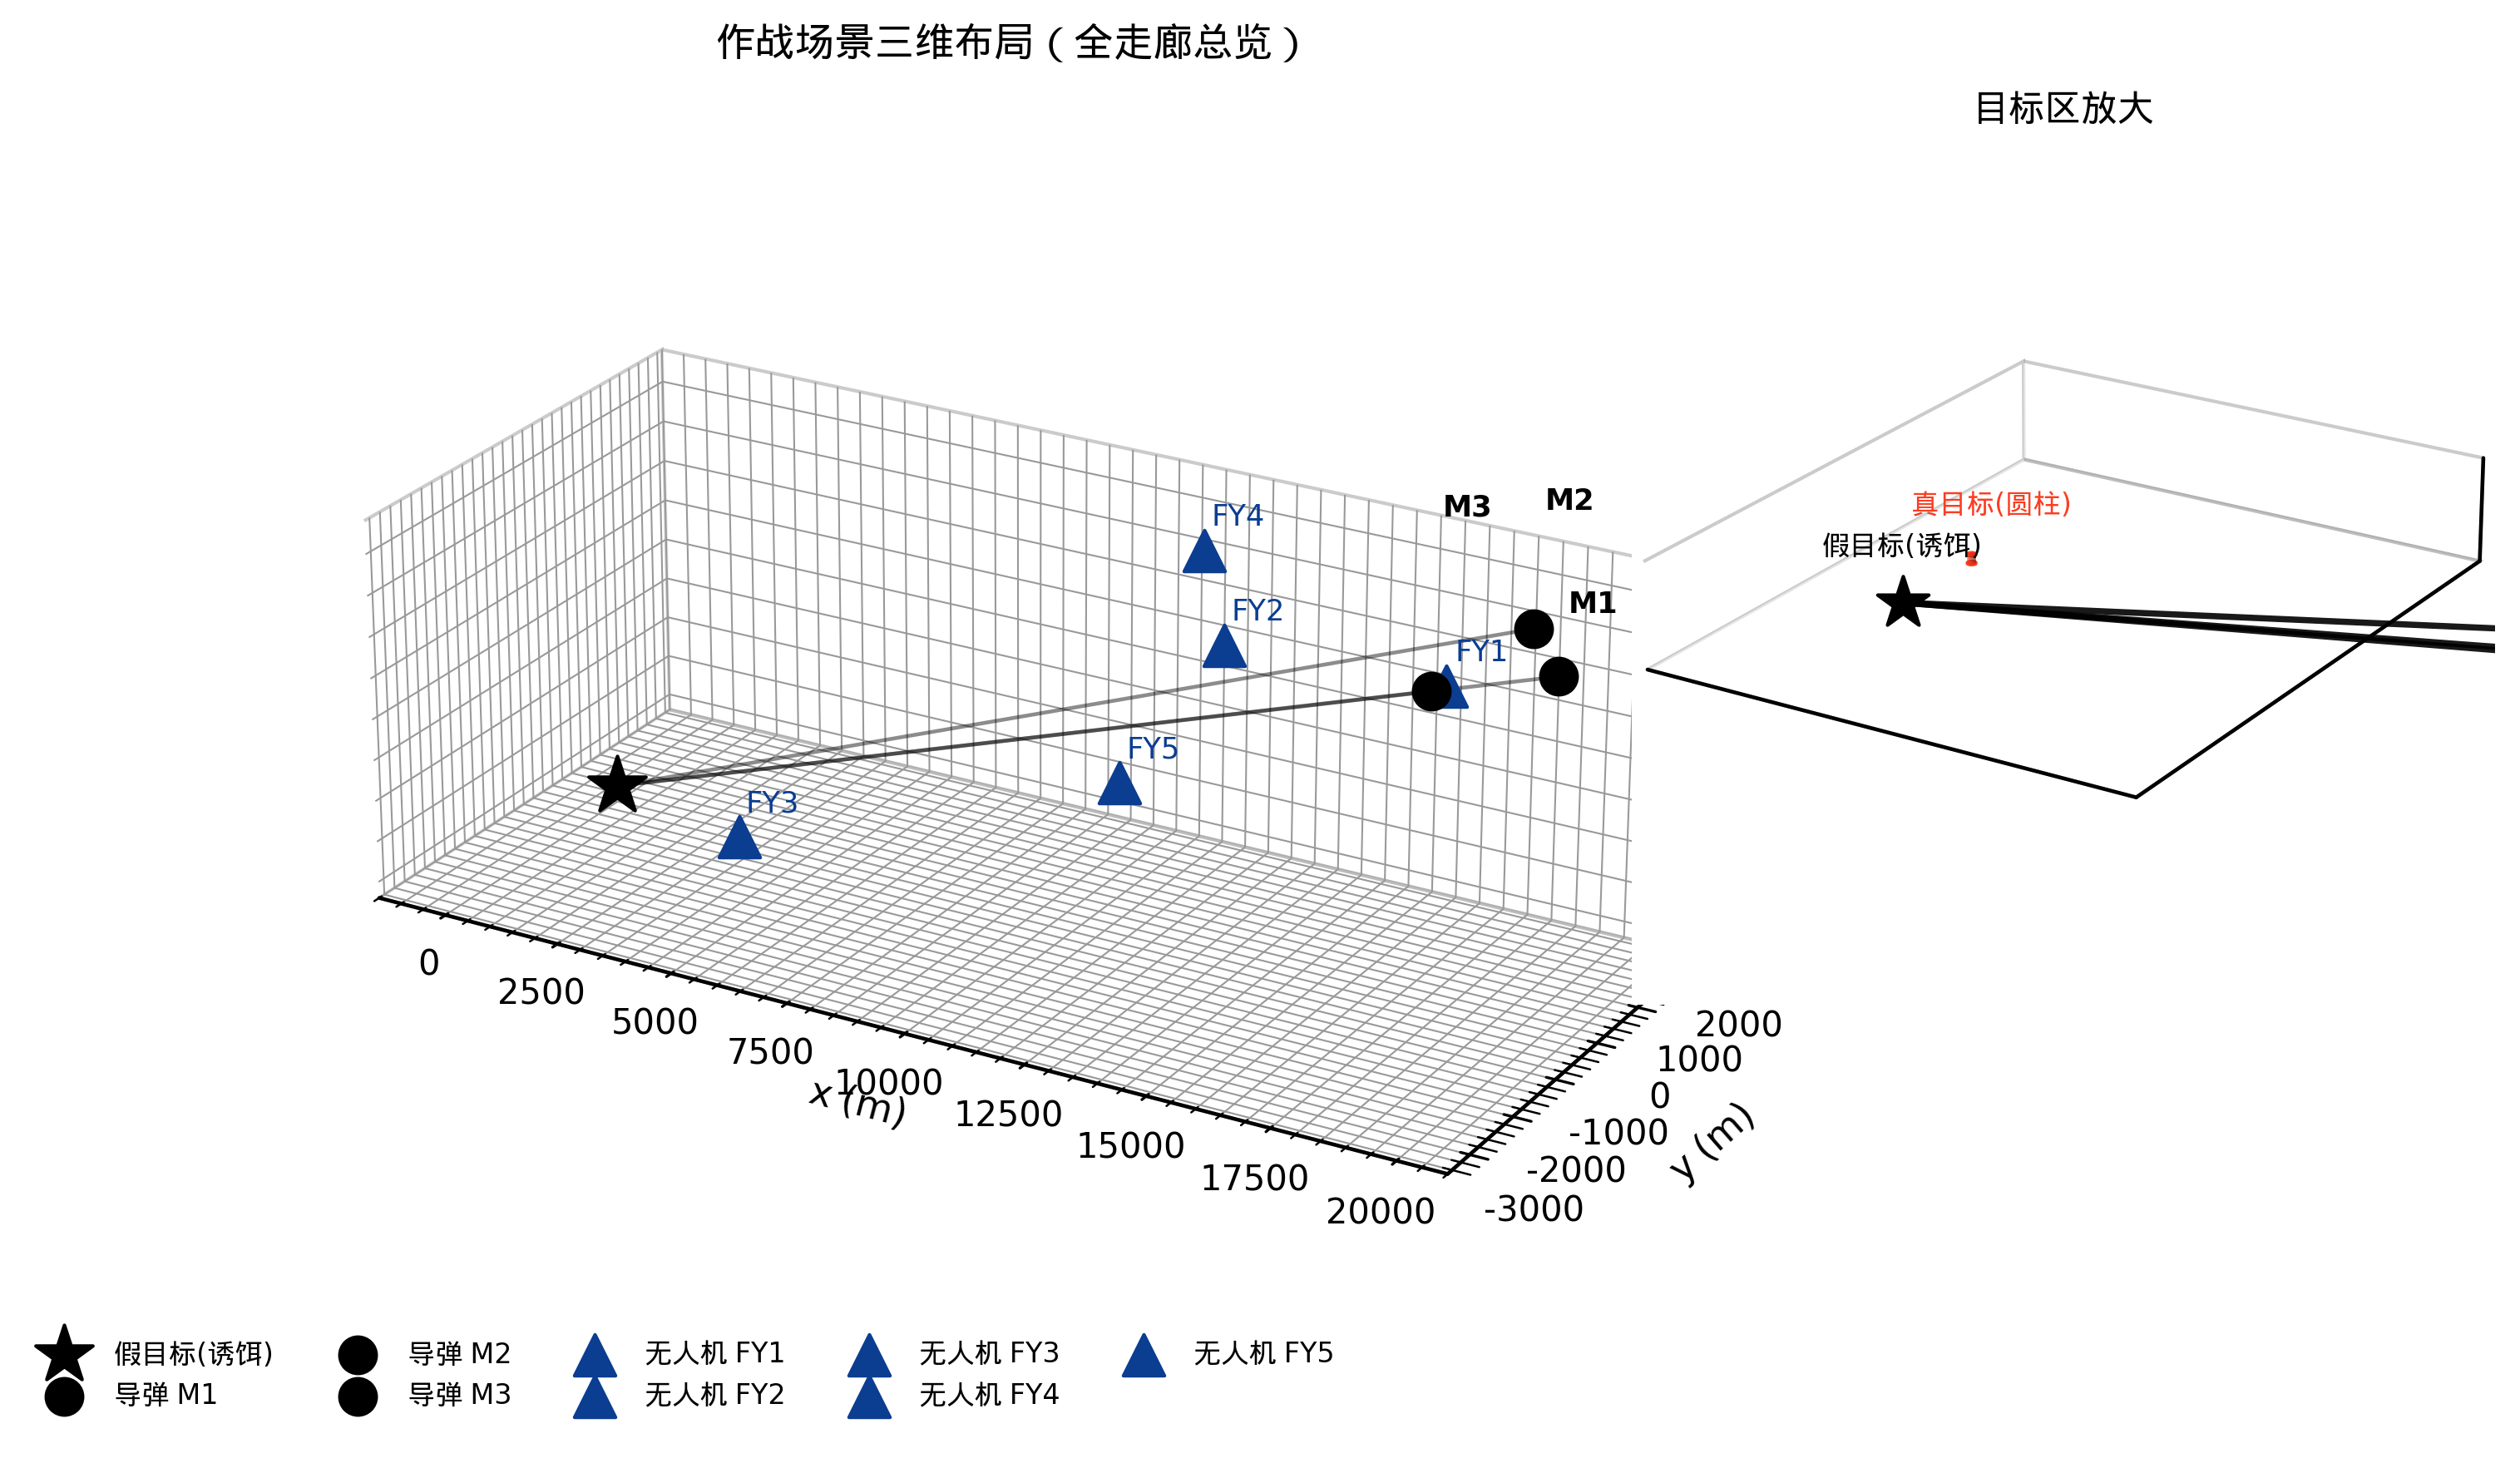
\includegraphics[width=\textwidth]{images/fig00_1_scene_3d.png}
\caption{作战场景三维布局：导弹、无人机与目标几何（左：全走廊总览；右上：目标区放大，圆柱目标以半透明实体表示）}
\label{fig:scene3d}
\end{minipage}
\end{figure}

\begin{figure}[H]
\centering
\begin{minipage}[t]{0.86\textwidth}
\centering
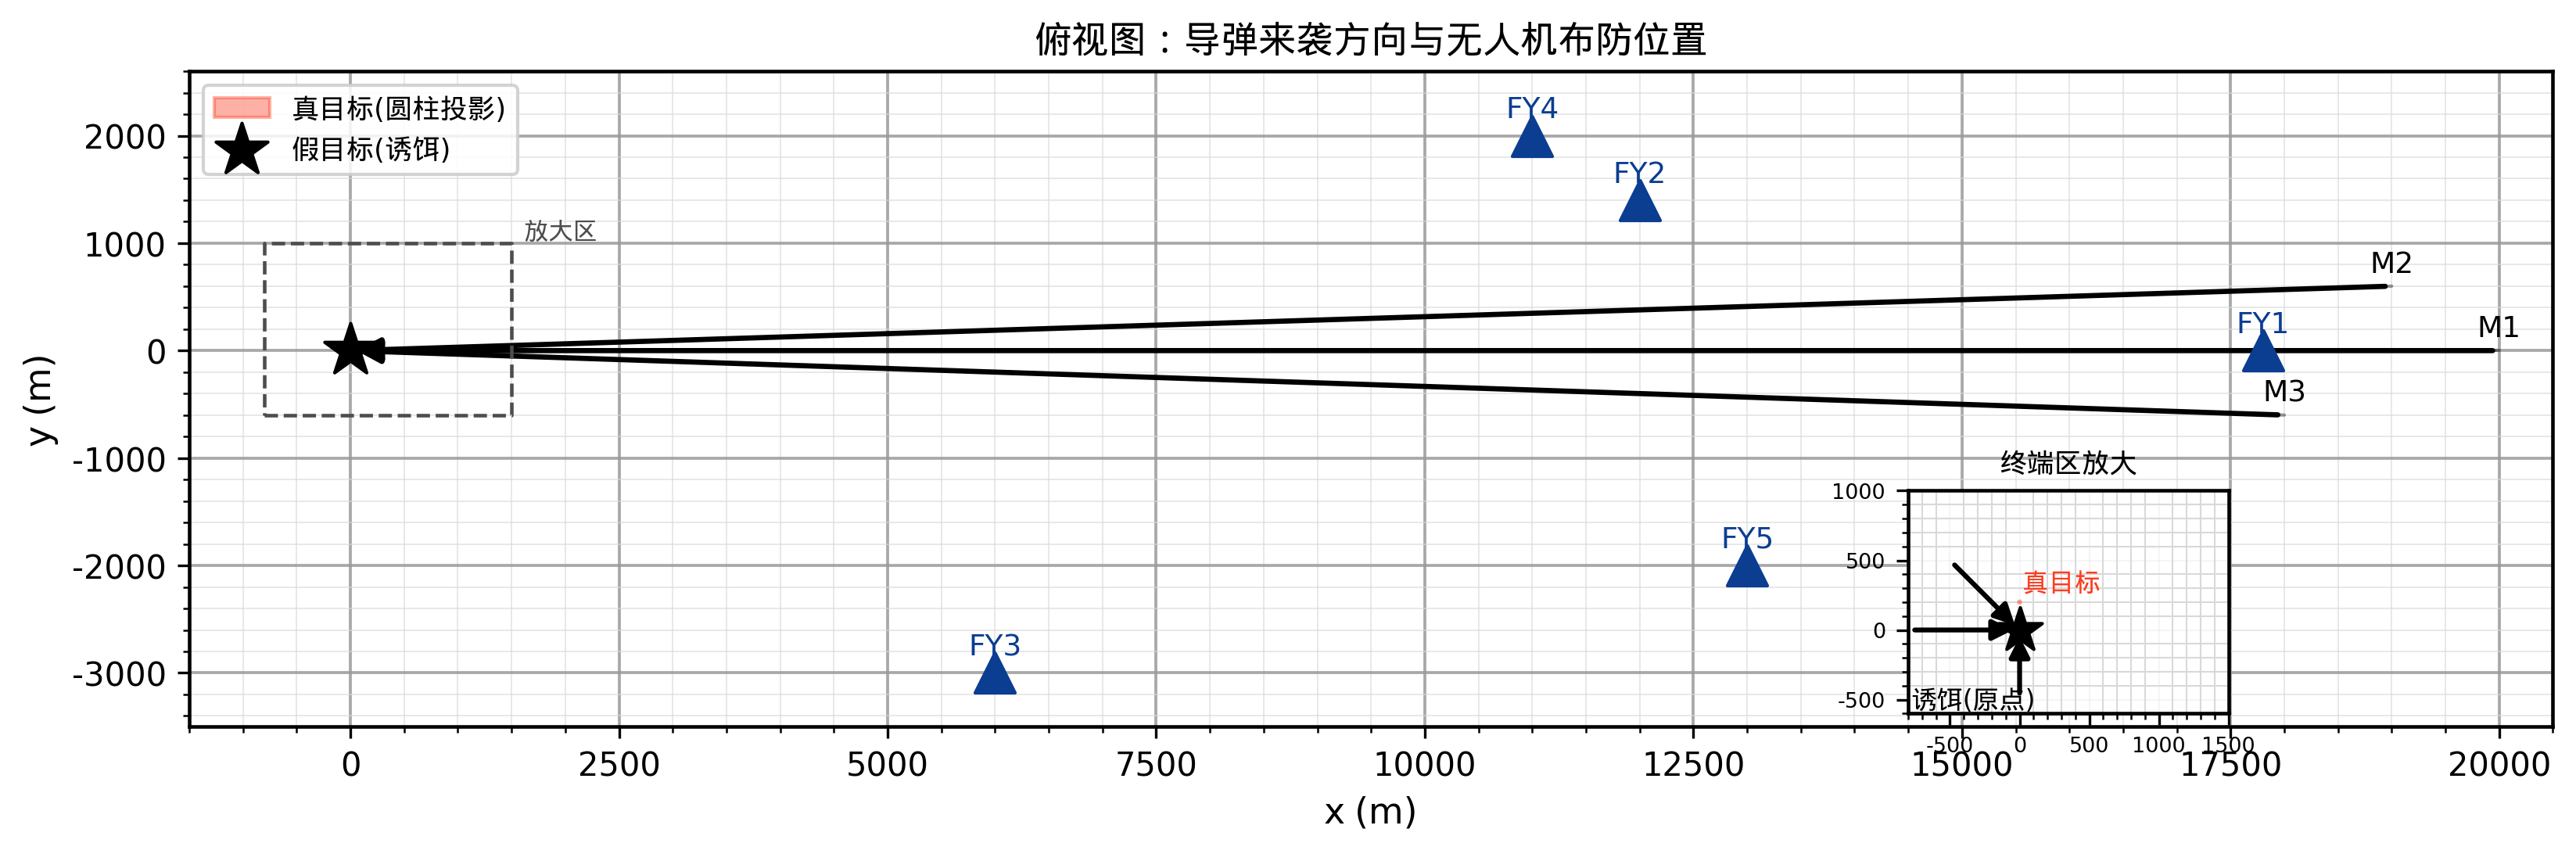
\includegraphics[width=\textwidth]{images/fig00_2_topview.png}
\caption{俯视图：导弹来袭方向与无人机布防位置（右下：终端区放大，目标/诱饵几何可见）}
\label{fig:topview}
\end{minipage}
\end{figure}
%% ==================== 3. 问题分析 ====================
\section{问题分析}

本问题在数学上是一个"确定性三维运动学仿真 + 连续/组合优化"的混合问题。导弹、无人机、
烟幕弹与云团的运动学关系均由题目给定参数唯一确定，不存在随机性，因此核心建模工作有两层：
一是建立精确的视线遮挡几何模型，把"有效遮蔽"翻译成可计算的数学判据；二是在该判据之上，
针对各问题不同的资源规模设计相应的优化算法。

\subsection{问题一、二分析}

问题一与问题二共享同一个单弹几何运动学模型，差别只在于投放策略是"给定"还是"待优化"。
问题一按给定参数正演计算云团轨迹并与导弹视线逐时刻比对，得到遮蔽时长，是整个模型体系的
校准性检验。问题二放开航向、速度、投放时刻与起爆延迟四个自由度，把"如何投放"转化为一个
4 维连续非线性规划；其难点在于遮蔽时长对参数呈分段结构、可行域极窄，需要结合物理直觉
构造初始解。

题目给出的全部输入（三枚导弹与五架无人机的位置、目标与诱饵几何、各物理参数）均为确定性
标量，无缺失与量纲冲突。建模前先把这些参数抽取为统一的场景配置，并做几何可视化核对：
三枚导弹到假目标的距离在 $18.1\sim20.1$ km 之间，按 $300$ m/s 计算约在 $60\sim67$ s 后
到达，这给出了投放窗口的时间上界；五架无人机距真目标 $6.8\sim17.9$ km 不等，其中 FY3
最接近真目标，为问题五的多机分工提供了空间上的天然差异。对问题二，决策变量为 FY1 的航向角、速度、
投放时刻与起爆延迟，共 4 维连续变量，目标函数为遮蔽时长，属于典型的连续非线性规划；由于
遮蔽时长对参数呈分段结构、可行域极窄，本文采用物理启发多起点配合坐标轮换精化的求解策略。
\subsection{问题三分析}

问题三把弹数放大到三枚，FY1 的航向与速度共用，三枚弹各有一组投放时刻与起爆延迟，共 8 维
变量，约束为相邻投放间隔不小于 1 s。这里的关键是把"间隔不小于 1 s"的不等式约束转化为
排序参数化，让优化器在无约束空间中搜索；目标取三弹遮蔽区间的并集测度，天然支持题目
"遮蔽可不连续"的要求。\subsection{问题四、五分析}

问题四让三架无人机各投 1 枚弹，共 12 维变量联合优化，属于多机协同问题，可看作问题五的
简化情形。问题五把规模扩展为 5 机 $\times$ 至多 3 弹 $\times$ 3 导弹，直接做数十维联合
全局优化既困难也缺乏可解释性，因此本文采用"单弹优化—贪心分配—局部精化"的分阶段框架，
把组合分配与连续优化分层解耦。对问题五，资源规模扩大为 5 机 $\times$ 至多 3 弹 $\times$ 3 导弹，直接
做数十维联合全局优化既困难也无必要，本文采用"单弹优化—贪心分配—局部精化"的分阶段框架：
先对每个（无人机，导弹）组合求单弹最优解，再在每机弹数、投放间隔约束下贪心挑选边际增益
最大的弹加入方案，最后对入选弹做局部精化。

五个子问题共用同一套几何运动学模型，这正是本文模型设计的核心思路：问题一、二共用
单弹正演与优化框架，问题三叠加投放时序与并集测度，问题四、五再加上多机协同与弹—导弹
分配，层次清晰、复用充分。从方法论看，本文要解决的是一个连续非线性规划与组合分配的
混合问题。连续层面选航向、速度与起爆延迟，组合层面排弹—导弹指派与投放时序，两者相互
耦合。纯解析方法难以刻画遮蔽时长的分段结构，纯元启发式又缺少可解释性。物理启发多起点
加坐标轮换精化，再配合分阶段的贪心分配框架，恰好在这两种极端之间取得了平衡。文献方面，烟幕遮蔽效应建模参考了烟幕干扰对制导系统
命中率影响的研究，弹道运动学参考了弹道闭式近似解的工作，连续优化采用差分进化范式与坐标
轮换精化相结合的策略，多机任务分配参考了多无人机系统任务分配与无人机路径规划的框架。

%% ==================== 4. 模型假设 ====================
\section{模型假设}

为使模型具有可操作性，结合题目的实际背景，本文提出以下假设：

\begin{enumerate}[label=\textbf{假设\arabic*：}, leftmargin=*]
    \item 导弹在来袭过程中始终沿直线飞向假目标，速度恒为 $300$ m/s，忽略重力对导弹弹道
          的影响。\textit{依据：}题目明确给出导弹飞行方向直指假目标且速度为常数，来袭段
          弹道可视为直线。
    \item 无人机受领任务后瞬时调整航向，之后等高度匀速直线飞行，速度与航向不再改变。
          \textit{依据：}题目原文规定。
    \item 烟幕干扰弹脱离无人机后仅受重力作用，初速等于无人机当时的速度矢量，忽略空气阻力
          与风场影响。\textit{依据：}题目只给出重力作用；对 $10\sim 20$ s 量级的弹道，
          空气阻力影响有限，且无风场数据可依。
    \item 烟幕云团为球状，起爆瞬时形成，此后以 $3$ m/s 匀速下沉，有效遮蔽半径为 $10$ m、
          有效时长为 $20$ s。\textit{依据：}题目给出的试验数据。
    \item 云团对导弹的遮蔽判据为：云团中心到"导弹—真目标参考点"视线线段的距离不超过
          $10$ m。\textit{依据：}云团中心 $10$ m 范围内浓度足以遮蔽的试验结论；参考点取
          真目标下底面圆心 $(0,200,0)$，其高度选择的敏感性在第 8 节考察。
    \item 多枚烟幕弹的遮蔽时间取各云团遮蔽区间的时间并集测度，遮蔽可以不连续。
          \textit{依据：}题目明确规定不同烟幕干扰弹的遮蔽可不连续。
    \item 各无人机的决策相互独立，同一无人机的航向与速度为其所有弹共用，相邻两弹投放间隔
          不小于 $1$ s。\textit{依据：}题目对每机航向速度"一旦确定不再调整"与投放间隔的规定。
\end{enumerate}

%% ==================== 5. 符号说明 ====================
\section{符号说明}

本文所用主要符号及其含义如表~\ref{tab:symbols}~所示。

\begin{table}[H]
\centering
\caption{主要符号说明}
\label{tab:symbols}
\begin{tabular}{cll}
\toprule
\textbf{符号} & \textbf{含义} & \textbf{单位} \\
\midrule
$M(t)$  & 导弹在 $t$ 时刻的位置矢量 & m \\
$F_0$   & 无人机初始位置 & m \\
$\theta$ & 无人机航向角（与 $+x$ 轴夹角，逆时针为正） & ${}^{\circ}$ \\
$v$     & 无人机飞行速度 & m/s \\
$t_{\mathrm{drop}}$ & 烟幕弹投放时刻（受领任务后） & s \\
$t_{\mathrm{delay}}$ & 投放至起爆的延迟时间 & s \\
$D$     & 投放点位置矢量 & m \\
$E$     & 起爆点位置矢量 & m \\
$C(t)$  & 云团中心在 $t$ 时刻的位置矢量 & m \\
$P_T$   & 真目标参考点 $(0,200,0)$ & m \\
$R$     & 云团有效遮蔽半径（$10$ m） & m \\
$\tau$  & 云团有效遮蔽时长（$20$ s） & s \\
$T_{\mathrm{shield}}$ & 有效遮蔽时间（多弹取并集测度） & s \\
$g$     & 重力加速度（$9.8$ m/s$^2$） & m/s$^2$ \\
\bottomrule
\end{tabular}
\end{table}
%% ==================== 6. 模型的建立与求解 ====================
\section{模型的建立与求解}

\subsection{共享几何运动学模型}

五问共用的核心模型由四条运动学链路与一条遮蔽判据构成。

\textbf{（1）导弹运动。}设导弹初始位置为 $M_0$，假目标位于原点，则导弹沿直线飞向假目标，
单位方向矢量 $\hat{u}=(O-M_0)/\|O-M_0\|$，$t$ 时刻位置为
\begin{equation}
    M(t) = M_0 + v_m\, t\, \hat{u},\qquad v_m = 300\ \text{m/s}.
    \label{eq:missile}
\end{equation}

\textbf{（2）无人机运动。}无人机等高度匀速直线飞行，$t$ 时刻位置为
\begin{equation}
    F(t) = F_0 + v\, t\, (\cos\theta,\ \sin\theta,\ 0),\qquad v\in[70,140]\ \text{m/s}.
    \label{eq:uav}
\end{equation}

\textbf{（3）烟幕弹弹道。}弹在 $t_{\mathrm{drop}}$ 时刻于 $D=F(t_{\mathrm{drop}})$ 投放，
初速为无人机水平速度 $v(\cos\theta,\sin\theta,0)$，此后仅受重力，投放后 $s$ 秒的位置为
\begin{equation}
    B(s) = D + v\, s\,(\cos\theta,\sin\theta,0) - \tfrac{1}{2} g s^2\,(0,0,1),
    \label{eq:ballistic}
\end{equation}
起爆点 $E = B(t_{\mathrm{delay}})$，起爆时刻 $t_{\mathrm{det}}=t_{\mathrm{drop}}+t_{\mathrm{delay}}$。

\textbf{（4）云团运动。}云团在起爆点瞬时形成并以 $3$ m/s 匀速下沉，起爆后 $\Delta t$ 秒
云团中心为
\begin{equation}
    C(t) = E - 3\,(t-t_{\mathrm{det}})\,(0,0,1),\qquad t\in[t_{\mathrm{det}},\ t_{\mathrm{det}}+\tau].
    \label{eq:cloud}
\end{equation}

\textbf{（5）遮蔽判据。}设 $\operatorname{dist}(P, \overline{AB})$ 表示点 $P$ 到线段
$\overline{AB}$ 的最短距离，$t$ 时刻云团对导弹 $m$ 形成有效遮蔽当且仅当
\begin{equation}
    \operatorname{dist}\!\big(C(t),\ \overline{M_m(t)\,P_T}\big) \leq R = 10\ \text{m},
    \label{eq:mask}
\end{equation}
其中 $\overline{M_m(t)\,P_T}$ 为导弹位置到真目标参考点的视线线段。采用点—线段距离而非
点—直线距离，是为了排除云团位于导弹后方或目标后方时"虽在直线上却并不遮挡"的情形。
对 $N$ 枚弹，设第 $i$ 枚弹在有效窗口内满足式~(\ref{eq:mask}) 的时间区间集合为
$\mathcal{I}_i=\bigcup_k[a_{ik},b_{ik}]$，则总有效遮蔽时长为
\begin{equation}
    T_{\mathrm{shield}} = \operatorname{meas}\!\Big(\bigcup_{i=1}^{N}\mathcal{I}_i\Big)
    = \sum_{k} \big(b_k - a_k\big),
    \label{eq:union}
\end{equation}
即各区间并集（合并重叠部分后）的总长度，天然支持"遮蔽可不连续"的要求。

式~(\ref{eq:mask}) 中的距离函数对时间连续，区间端点由"细采样检测符号变化 + 二分精化"
确定：先以 $0.02$ s 步长向量化计算距离序列，标记满足判据的连续段，再在每段两端用二分法
求出 $\operatorname{dist}=R$ 的精确时刻，从而得到高精度的遮蔽区间。该实现同时保证了
优化器高频调用时的计算效率。视线遮挡判据的几何含义如图~\ref{fig:los}~所示：烟幕云团
（有效半径 $10$ m 的球体）位于导弹与真目标之间的视线附近时，导弹的探测视线被遮蔽。

\begin{figure}[H]
\centering
\begin{minipage}[t]{0.86\textwidth}
\centering
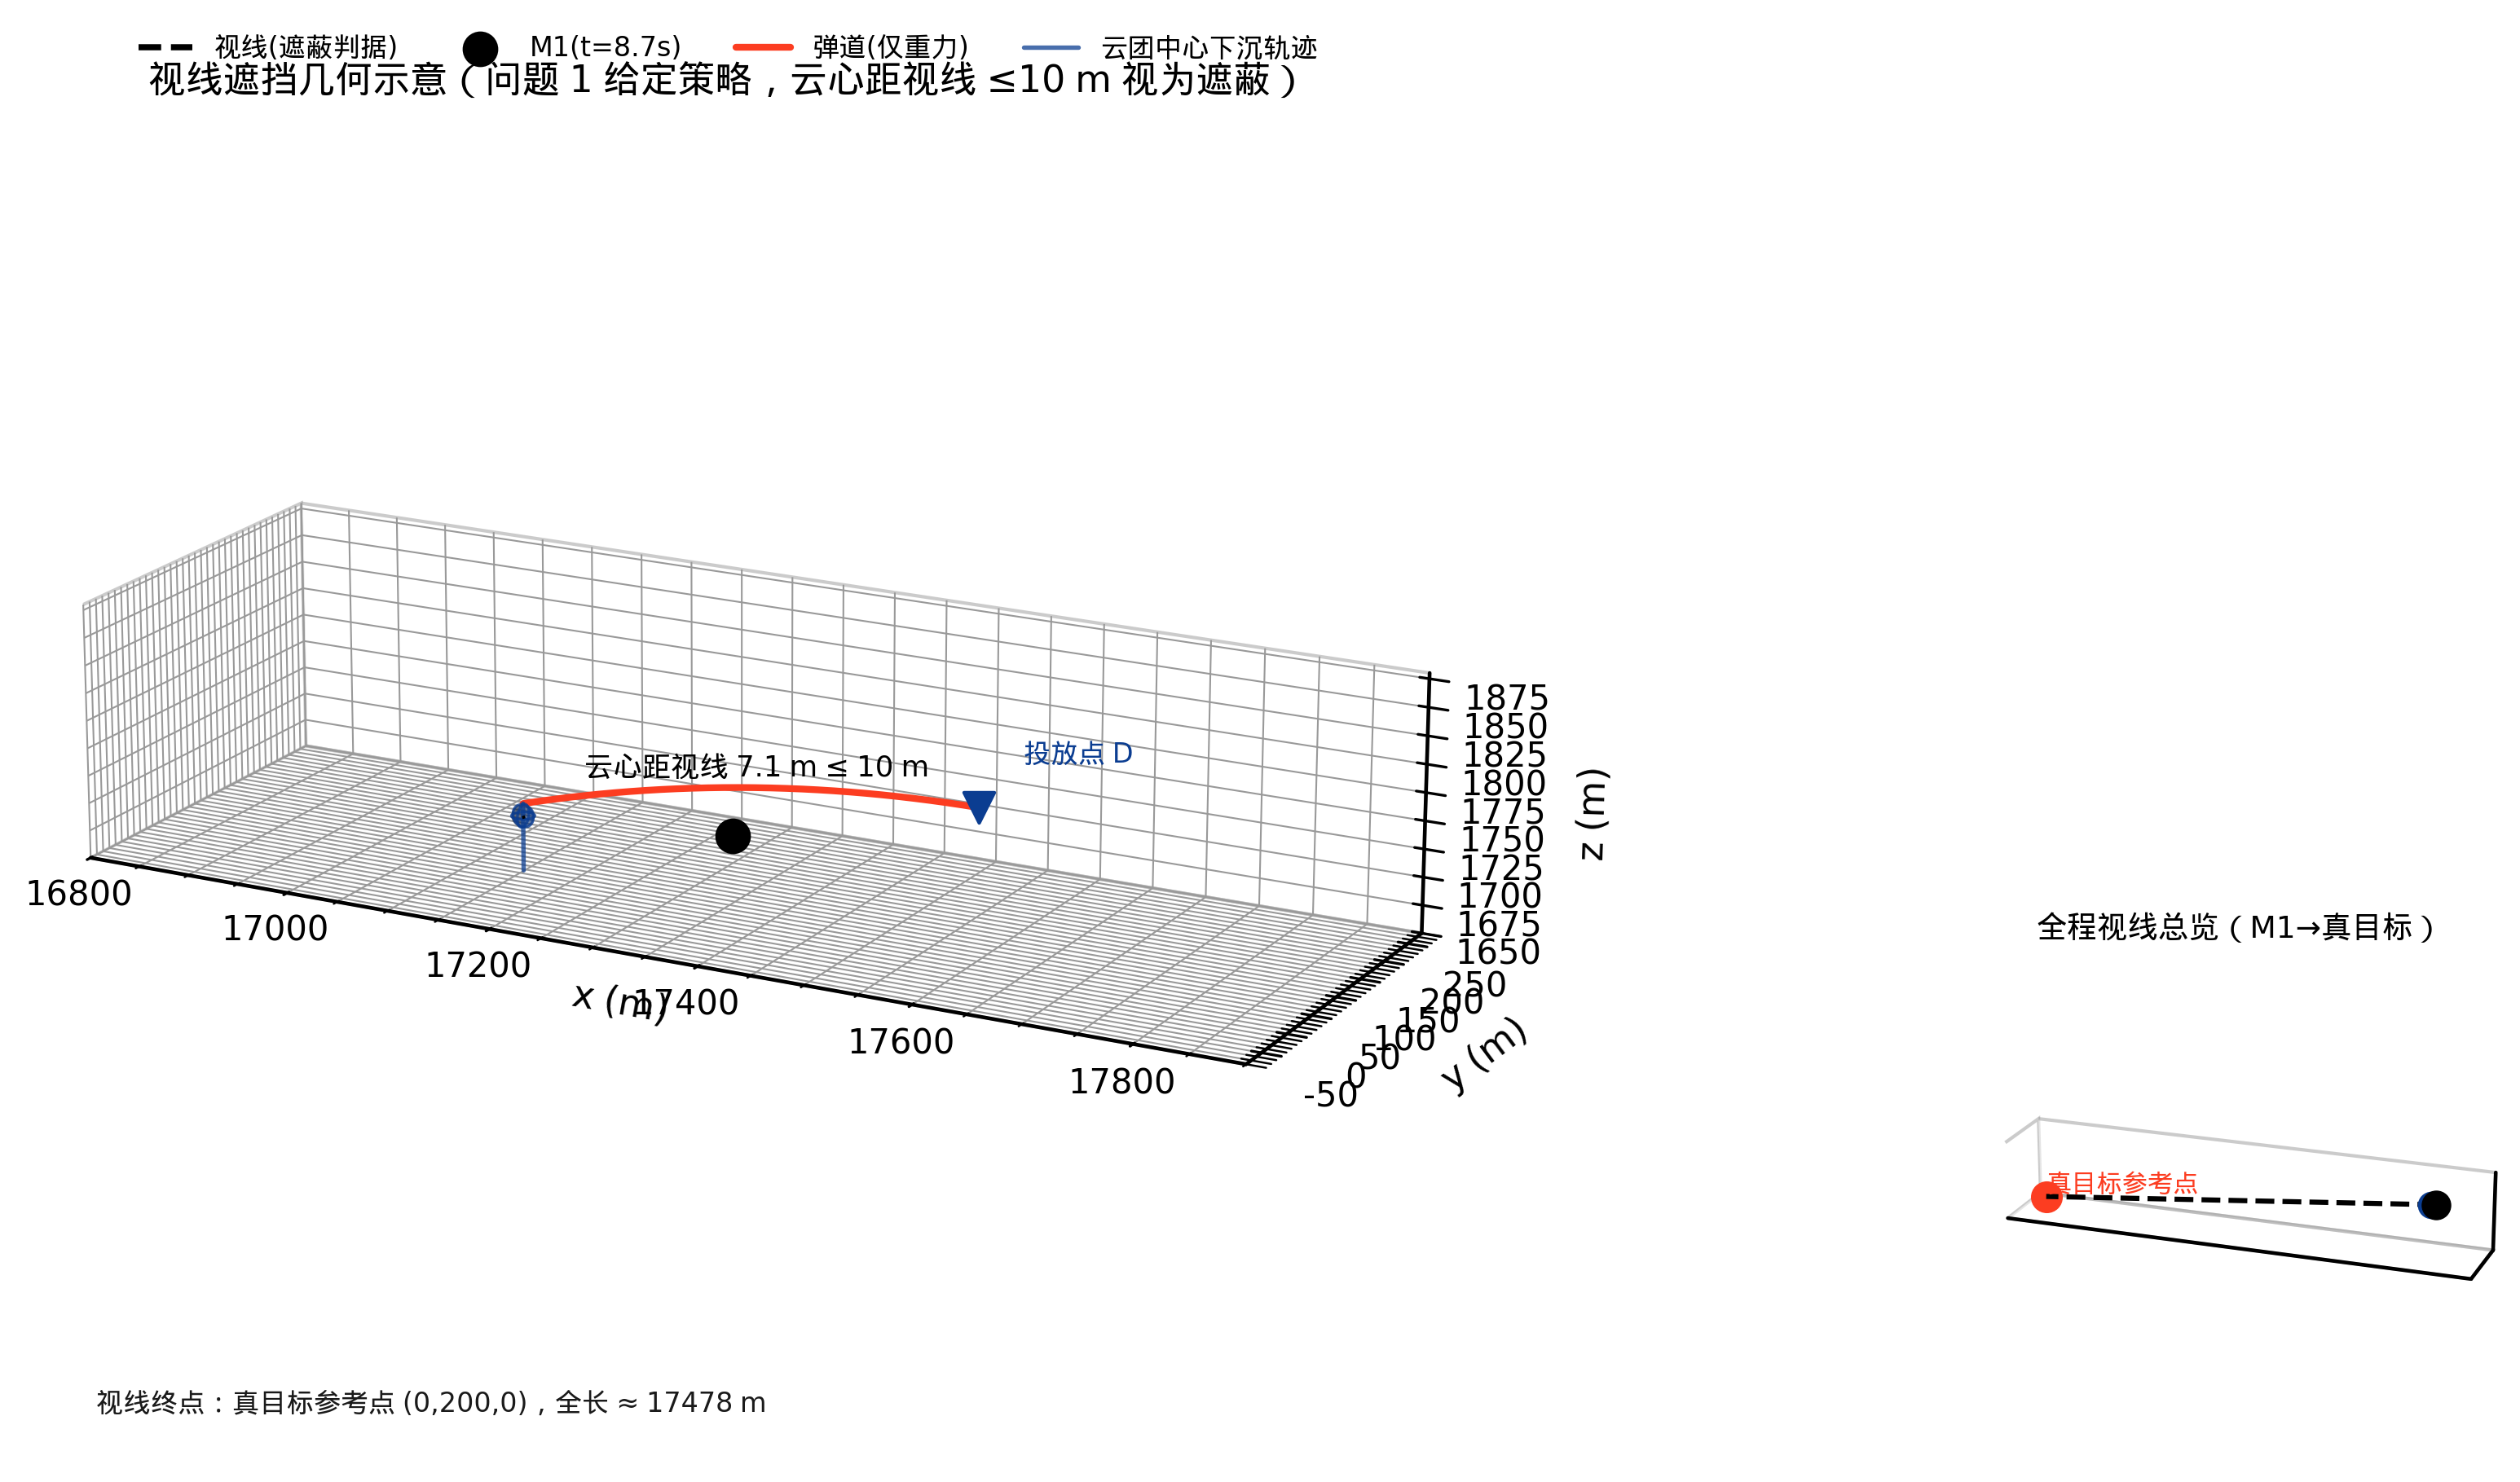
\includegraphics[width=\textwidth]{images/fig00_3_los_geometry.png}
\caption{视线遮挡几何示意（问题 1 给定策略：云心距视线线段 $\leq 10$ m 视为遮蔽，图上直接标注实际距离；右下为全程视线总览）}
\label{fig:los}
\end{minipage}
\end{figure}

上述模型的数值实现还有两个值得说明的要点。其一是向量化：遮蔽判据需要在每个时间步
对每条视线计算一次点—线段距离，优化器一次目标函数求值就要扫描上千个时间步，逐点循环
会使单次求值达到数十毫秒、整个优化不可行；实现中把全部时间步的距离计算写成向量化的
矩阵运算，单次目标函数求值降至约 1 毫秒量级，使多起点精化流程能够在合理时间内完成。
其二是时间步长独立性：遮蔽区间端点用二分法精化到 $\operatorname{dist}=R$ 的精确时刻，
区间长度对采样步长不敏感——用 $0.02$ s 与 $0.005$ s 步长分别计算问题一，结果完全一致，
证明数值实现无网格依赖。

\subsection{问题一：给定策略的有效遮蔽时长}

问题一的投放策略完全给定：FY1 以 $120$ m/s 朝假目标方向飞行（水平方向角 $\theta=180^{\circ}$），
受领任务 $t_{\mathrm{drop}}=1.5$ s 后投放，$t_{\mathrm{delay}}=3.6$ s 后起爆。将参数代入
式~(\ref{eq:missile})—(\ref{eq:mask}) 正演计算，结果如表~\ref{tab:q1}~所示。

\begin{table}[H]
\centering
\caption{问题一给定策略的正演计算结果}
\label{tab:q1}
\begin{tabular}{lcc}
\toprule
\textbf{量} & \textbf{数值} & \textbf{说明} \\
\midrule
投放点 $D$ & $(17620.0,\ 0.0,\ 1800.0)$ m & $t=1.5$ s 时 FY1 位置 \\
起爆点 $E$ & $(17188.0,\ 0.0,\ 1736.5)$ m & 弹道 $t_{\mathrm{delay}}=3.6$ s \\
起爆时刻 & $5.10$ s & \\
遮蔽时间区间 & $[8.04,\ 9.45]$ s & 起爆后 $20$ s 窗口内 \\
\textbf{有效遮蔽时长} & \textbf{$1.410$ s} & \\
\bottomrule
\end{tabular}
\end{table}

可见给定策略下，云团在起爆后约 $3$ s 才开始进入视线 $10$ m 遮蔽带，且窗口较短：该策略中
FY1 的飞行方向与速度是"默认"选择，并未针对视线遮挡几何进行优化，因此遮蔽时长有限，这为
问题二的优化提供了明确的改进空间。

从机理上看，这段窗口由两种几何过程叠加而成：窗口起点对应导弹视线扫入云团 $10$ m 遮蔽带，
终点则对应导弹飞抵云团附近（云团距导弹自身小于 $10$ m）之后的脱离。值得说明的是，由于
导弹沿直线飞向假目标而真目标位于假目标正 $y$ 方向 $200$ m 处，视线在云团所在高度处是
近似固定的竖直平面内缓慢扫掠的，扫掠速度约每秒数米，这决定了单枚云团能够提供的遮蔽
时长存在一个自然的数量级上限，也为问题三至问题五"用多枚云团接力"的必要性提供了依据。

\subsection{问题二：单机单弹投放策略优化}

问题二在共享模型上叠加连续优化层。决策变量为
\begin{equation}
    x = (\theta,\ v,\ t_{\mathrm{drop}},\ t_{\mathrm{delay}}),
    \qquad \theta\in[0^{\circ},360^{\circ}),\ v\in[70,140],\ t_{\mathrm{drop}}\in[0,40],\
    t_{\mathrm{delay}}\in[0.5,15],
    \label{eq:q2var}
\end{equation}
目标函数为
\begin{equation}
    \max_{x}\ T_{\mathrm{shield}}(x) = \operatorname{meas}\!\big(\mathcal{I}(x)\big),
    \label{eq:q2obj}
\end{equation}
其中 $\mathcal{I}(x)$ 为式~(\ref{eq:mask}) 确定的单弹遮蔽区间。

由于遮蔽时长对参数呈分段常数—线性结构，且"云团恰好进入视线 $10$ m 带"的参数区域在
4 维空间中是一条狭窄管状邻域，直接从随机初始种群出发的全局优化几乎必然落入零值平原。
为此本文设计了两级求解策略：
\begin{enumerate}[label=\textbf{Step \arabic*：}, leftmargin=*]
    \item \textbf{物理启发多起点}：对一组候选遮蔽时刻 $t_m$ 与云团高度 $z$，把云团直接放在
          该时刻的视线 $M(t_m)\to P_T$ 上，再由弹道公式反解出 $(\theta,v,t_{\mathrm{drop}},
          t_{\mathrm{delay}})$，共生成数百个互不相同的可行起点；
    \item \textbf{两级坐标轮换精化}：对每个起点依次做 $\pm5\%$ 邻域与 $\pm1\%$ 邻域的
          逐变量网格扫描（坐标轮换爬山），先粗后细，取全部起点中的最优结果。
\end{enumerate}
优化结果如表~\ref{tab:q2}~所示，问题二将遮蔽时长由 $1.410$ s 提升至 $4.611$ s，提升约
$3.2$ s。最优解中 FY1 仍基本沿 $-\!x$ 方向（$\theta\approx178.5^{\circ}$）飞行，但速度降低到
约 $101$ m/s、投放时刻提前到受领任务后 $0.09$ s，起爆延迟约 $2.9$ s，使云团起爆后恰好位于
视线附近，遮蔽窗口由 $[3.64,8.25]$ s 的视线扫掠过程构成。

\begin{table}[H]
\centering
\caption{问题二单机单弹优化结果}
\label{tab:q2}
\begin{tabular}{lcc}
\toprule
\textbf{量} & \textbf{数值} & \textbf{说明} \\
\midrule
航向角 $\theta$ & $178.513^{\circ}$ & \\
速度 $v$ & $101.388$ m/s & \\
投放时刻 $t_{\mathrm{drop}}$ & $0.087$ s & \\
起爆延迟 $t_{\mathrm{delay}}$ & $2.904$ s & \\
投放点 $D$ & $(17791.2,\ 0.2,\ 1800.0)$ m & \\
起爆点 $E$ & $(17496.9,\ 7.9,\ 1758.7)$ m & \\
遮蔽时间区间 & $[3.64,\ 8.25]$ s & \\
\textbf{有效遮蔽时长} & \textbf{$4.611$ s} & 问题一提升 $+227\%$ \\
\bottomrule
\end{tabular}
\end{table}

最优解的结构值得解读。航向角 $178.5^{\circ}$ 意味着 FY1 几乎正对来袭方向飞行，这与直觉
一致——云团必须落在导弹与真目标之间的视线上，而 FY1 的初始位置恰好在 M1 来袭路径附近；
速度取 $101$ m/s 而非上限 $140$ m/s，是因为过快的速度会使云团在起爆时过于深入来袭方向，
偏离视线所在的高度带；投放时刻几乎为零、起爆延迟约 $2.9$ s，则让云团尽可能早地在视线
附近成形并随视线扫掠维持遮蔽。遮蔽窗口 $[3.64,8.25]$ s 的中段对应视线扫过云团的时段，
两端则分别由云团起爆时刻与导弹飞抵云团附近的时刻界定。

\begin{figure}[H]
\centering
\begin{minipage}[t]{0.86\textwidth}
\centering
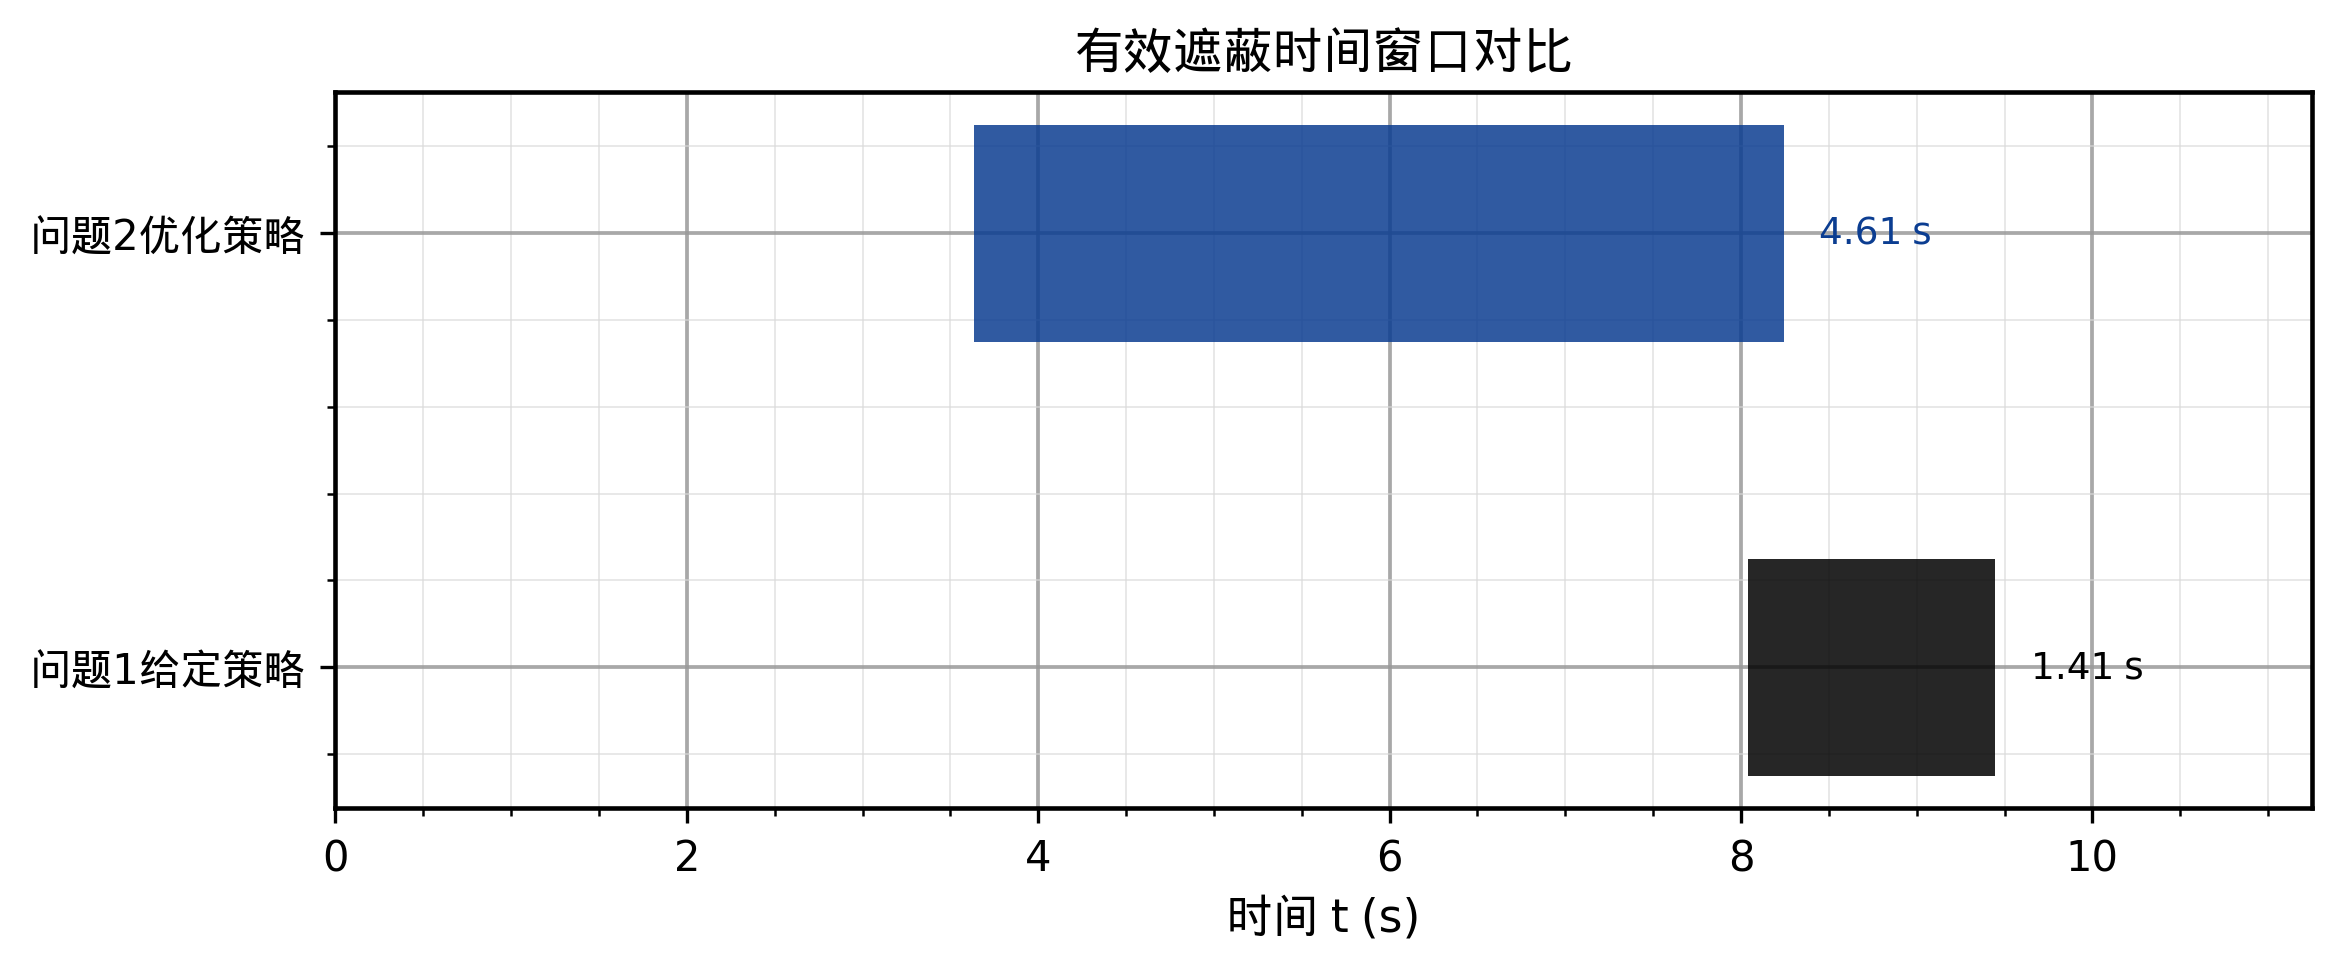
\includegraphics[width=\textwidth]{images/fig01_masking_window.png}
\caption{问题一与问题二遮蔽时间窗口对比（条形末端标注遮蔽时长）}
\label{fig:q1q2window}
\end{minipage}
\end{figure}

\begin{figure}[H]
\centering
\begin{minipage}[t]{0.86\textwidth}
\centering
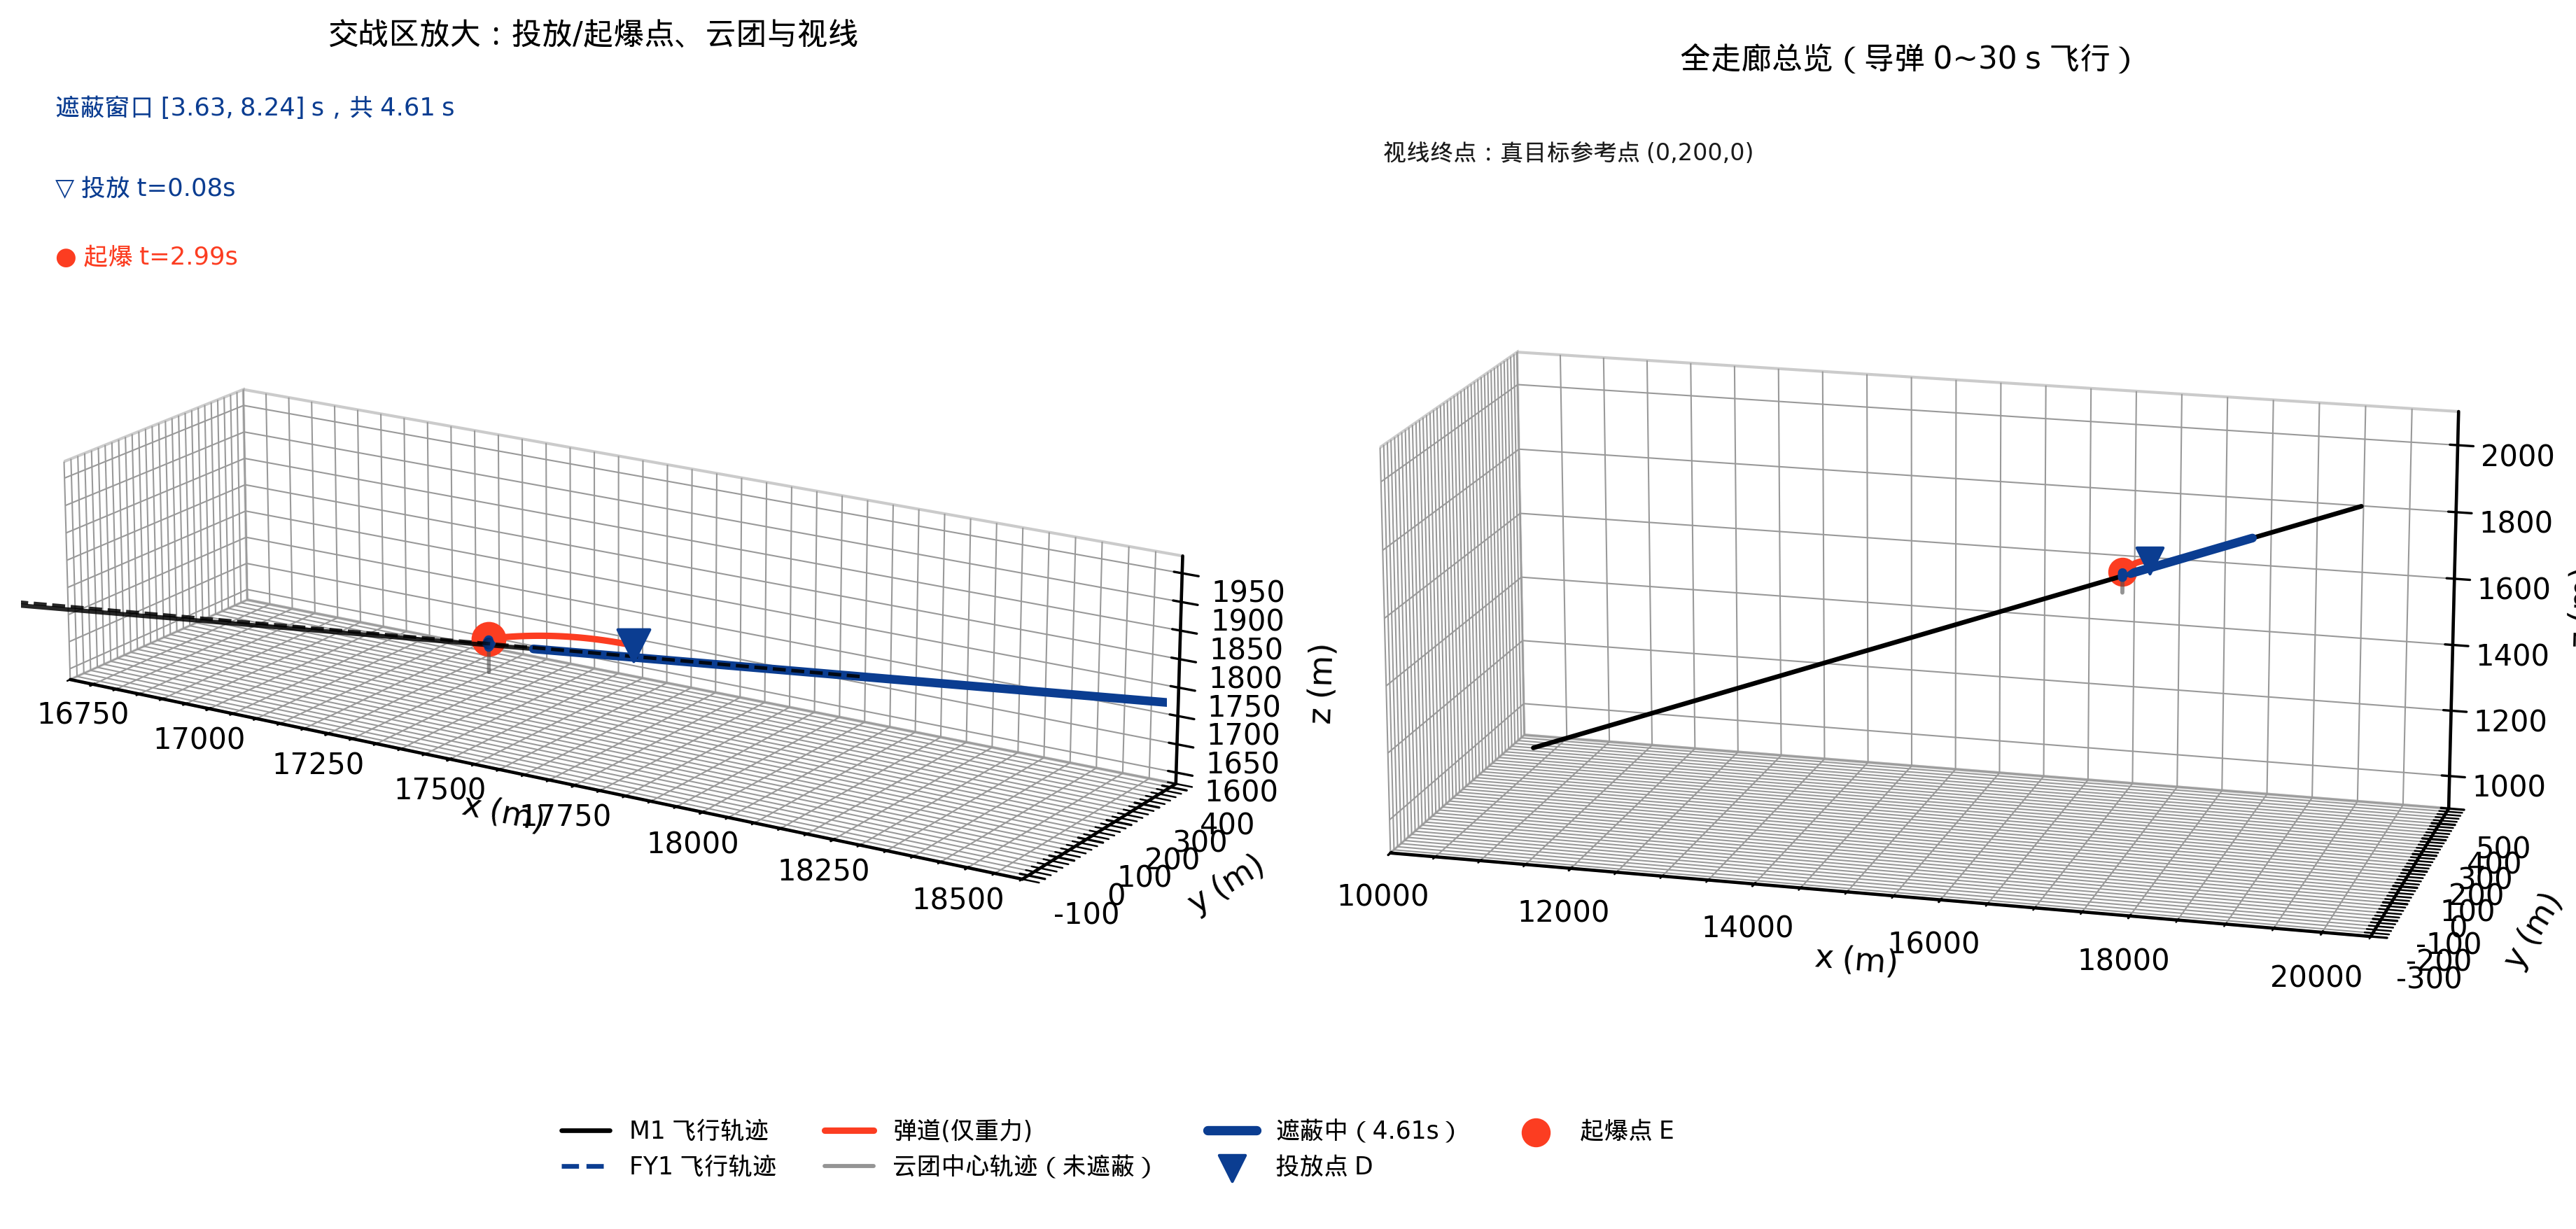
\includegraphics[width=\textwidth]{images/fig01_q2_trajectory.png}
\caption{问题二最优解的三维轨迹（左：交战区放大，投放/起爆关键时刻、云团与视线关系可读；右：全走廊总览；云团中心下沉轨迹中实际产生遮蔽的时间段高亮）}
\label{fig:q2traj}
\end{minipage}
\end{figure}

\subsection{问题三：单机三弹投放时序优化}

问题三中 FY1 的航向角与速度对所有三枚弹共用，第 $i$ 枚弹的投放时刻 $t_i$ 与起爆延迟
$d_i$ 独立，约束为相邻投放间隔不小于 $1$ s。为把不等式约束转化为变量取值范围，采用排序
参数化
\begin{equation}
    t_2 = t_1 + 1 + g_2,\qquad t_3 = t_2 + 1 + g_3,\qquad g_2,g_3 \geq 0,
    \label{eq:order}
\end{equation}
决策变量共 8 维 $x=(\theta,v,t_1,g_2,g_3,d_1,d_2,d_3)$，目标函数为三弹遮蔽区间并集测度。
求解仍采用物理启发多起点 + 两级坐标轮换精化：种子生成时沿 FY1 飞行射线按"视线自然高度
（在高度 $z$ 处视线近似位于 $x\approx10z$ 的竖直线上）"等距布设三枚云团，再反解各自的
投放时刻与起爆延迟，保证三弹的遮蔽窗口在时间上依次衔接。优化结果如表~\ref{tab:q3}~所示，
三弹遮蔽窗口分别为 $[5.23,8.63]$、$[8.42,11.03]$、$[11.03,12.49]$ s，前后基本衔接，
并集遮蔽时长 $7.263$ s，显著优于单弹最优的 $4.611$ s。

\begin{table}[H]
\centering
\caption{问题三单机三弹投放策略（FY1，结果已写入 result1.xlsx）}
\label{tab:q3}
\begin{tabular}{lcccc}
\toprule
\textbf{弹号} & $t_{\mathrm{drop}}$ (s) & $t_{\mathrm{delay}}$ (s) & 遮蔽区间 (s) & 单弹时长 (s) \\
\midrule
1 & $0.669$ & $4.186$ & $[5.23,\ 8.63]$ & $3.406$ \\
2 & $2.967$ & $4.890$ & $[8.42,\ 11.03]$ & $2.614$ \\
3 & $5.144$ & $5.889$ & $[11.03,\ 12.49]$ & $1.459$ \\
\midrule
\multicolumn{4}{l}{航向角 $\theta=179.640^{\circ}$，速度 $v=138.365$ m/s} &
\textbf{并集 $7.263$ s} \\
\bottomrule
\end{tabular}
\end{table}

三枚弹的投放时刻依次为 $0.669$、$2.967$、$5.144$ s，起爆延迟依次增大，使得三团烟雾
在空间上沿来袭方向错落排布、在时间上首尾相接：第一枚云团覆盖早期窗口，第二枚在它下沉
出遮蔽带之前接续，第三枚继续把窗口向后延伸。需要指出的是，三枚弹共用同一航向与速度，
云团只能沿 FY1 的飞行射线排布，因此并集时长并非单弹时长的简单三倍——后两枚弹的窗口
明显短于第一枚，这正是"共用航向约束"带来的物理代价，也是问题四改用多机协同、各机自由
选择航向后总时长得以大幅提升的原因。

三枚弹的投放点与起爆点坐标列于表~\ref{tab:q3coord}，供 result1.xlsx 回填核对。

\begin{table}[H]
\centering
\caption{问题三三枚弹的投放点与起爆点坐标（m）}
\label{tab:q3coord}
\begin{tabular}{lccc}
\toprule
\textbf{弹号} & \textbf{投放点} & \textbf{起爆点} & \textbf{起爆时刻 (s)} \\
\midrule
1 & $(17707.4,\ 0.6,\ 1800.0)$ & $(17128.3,\ 4.2,\ 1714.2)$ & $4.86$ \\
2 & $(17389.4,\ 2.6,\ 1800.0)$ & $(16712.8,\ 6.8,\ 1682.8)$ & $7.86$ \\
3 & $(17088.3,\ 4.5,\ 1800.0)$ & $(16273.5,\ 9.6,\ 1630.1)$ & $11.03$ \\
\bottomrule
\end{tabular}
\end{table}

\begin{figure}[H]
\centering
\begin{minipage}[t]{0.86\textwidth}
\centering
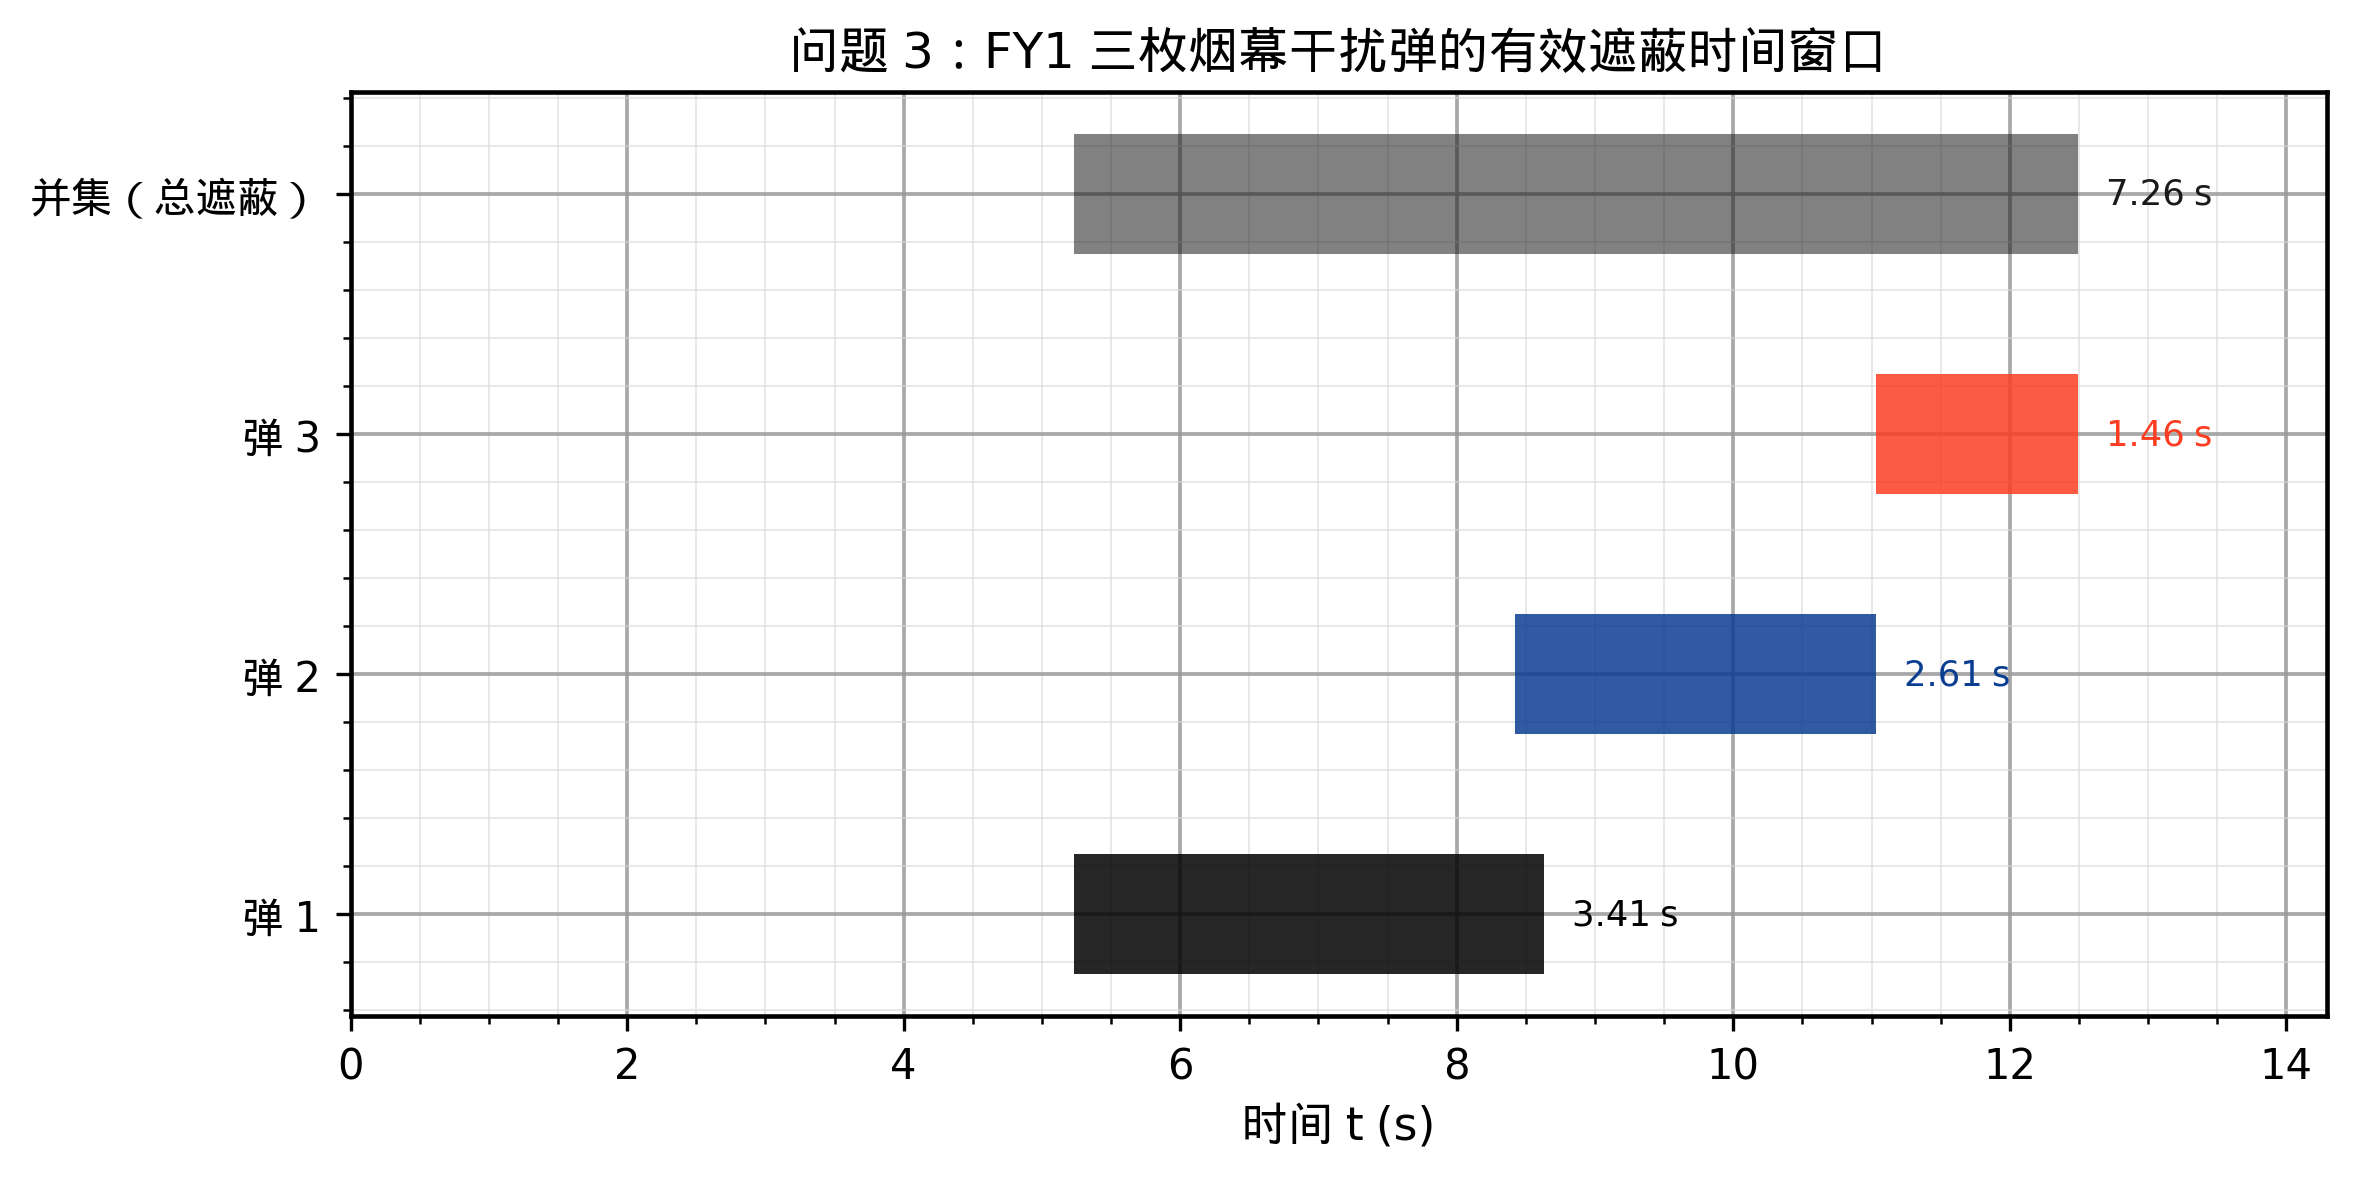
\includegraphics[width=\textwidth]{images/fig02_q3_masking_window.png}
\caption{问题三三枚烟幕弹的有效遮蔽时间窗口（末行为并集，条形末端标注各弹时长）}
\label{fig:q3window}
\end{minipage}
\end{figure}

\subsection{问题四：三机协同投放优化}

问题四让 FY1、FY2、FY3 各投放 1 枚弹干扰 M1，三机的航向、速度、投放时刻与起爆延迟均
可独立选择，共 12 维变量，目标取三枚弹对 M1 遮蔽区间的并集测度。求解分两步走：先对每架
无人机单独做单弹优化得到候选解，再以多组联合起点（单弹最优组合及其抖动、错峰变换）
做联合坐标轮换精化。优化结果见表~\ref{tab:q4}。三机遮蔽区间相互分离，并集遮蔽时长达到
$15.354$ s，约为单机三弹方案的 $2.1$ 倍——多机协同的价值正在于此：不同空间位置的无人机
能够在来袭时段上错峰接力，把遮蔽窗口显著拉长。

\begin{table}[H]
\centering
\caption{问题四三机协同投放策略（结果已写入 result2.xlsx）}
\label{tab:q4}
\begin{tabular}{lcccccc}
\toprule
\textbf{无人机} & $\theta$ (${}^{\circ}$) & $v$ (m/s) & $t_{\mathrm{drop}}$ (s) & $t_{\mathrm{delay}}$ (s) & 单弹时长 (s) \\
\midrule
FY1 & $176.98$ & $71.02$ & $0.02$ & $2.52$ & $4.676$ \\
FY2 & $239.20$ & $139.97$ & $3.72$ & $7.44$ & $4.986$ \\
FY3 & $135.54$ & $139.96$ & $22.88$ & $9.16$ & $5.691$ \\
\midrule
\multicolumn{6}{l}{\textbf{三机并集遮蔽时长 $15.354$ s}} \\
\bottomrule
\end{tabular}
\end{table}

\begin{figure}[H]
\centering
\begin{minipage}[t]{0.86\textwidth}
\centering
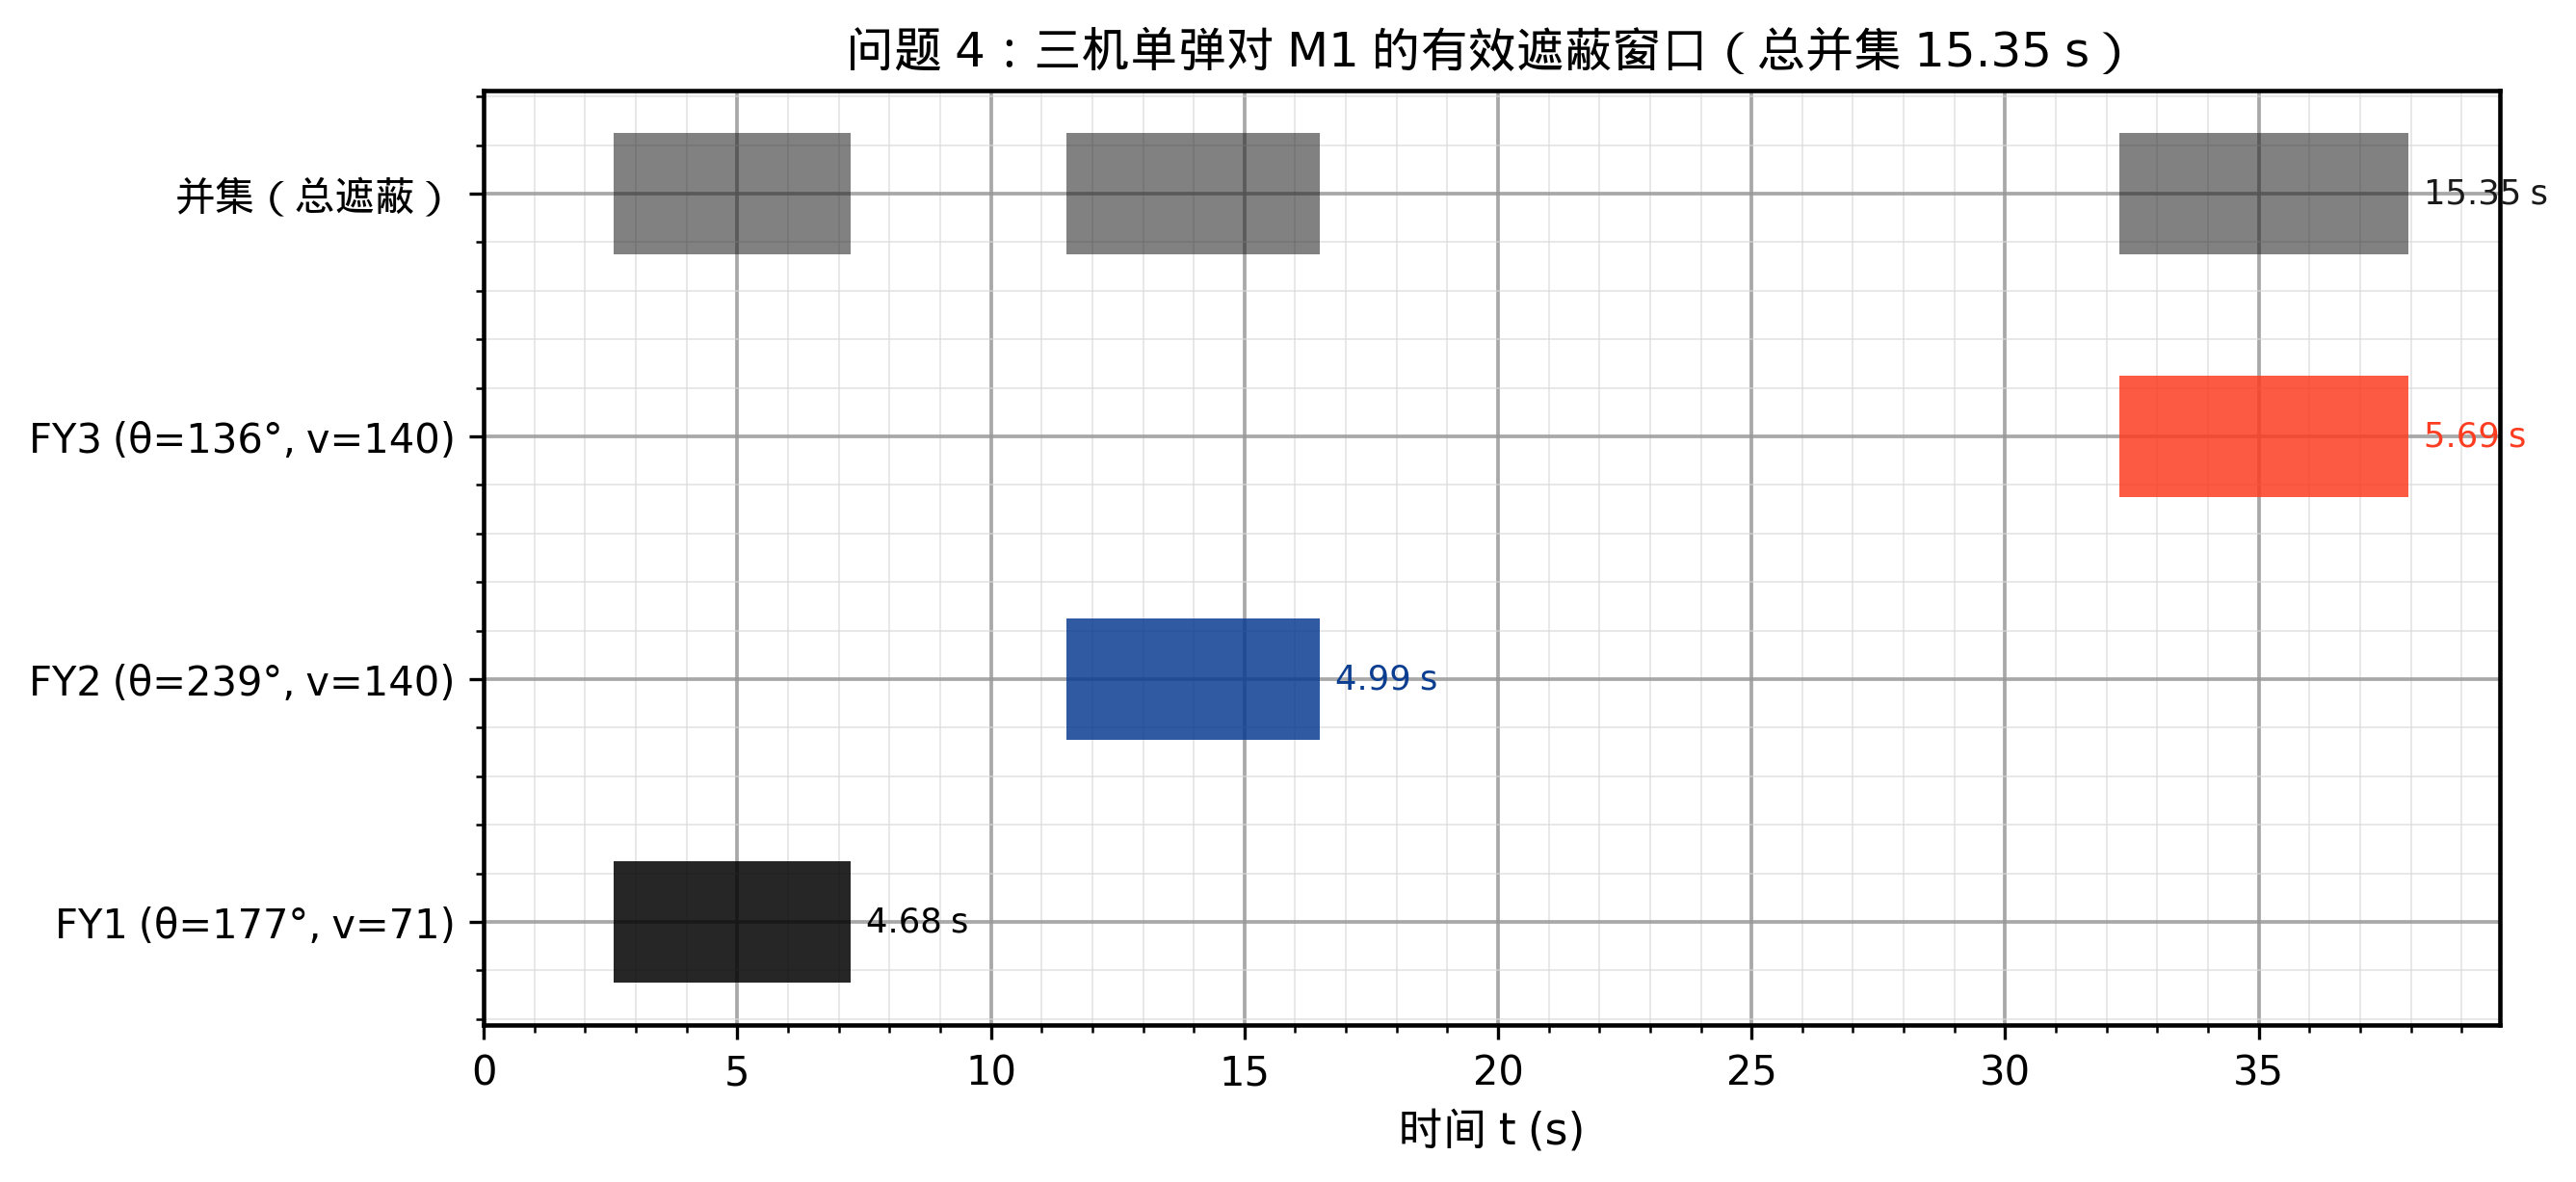
\includegraphics[width=\textwidth]{images/fig03_q4_masking_window.png}
\caption{问题四三机投放的遮蔽时间窗口（末行为并集，条形末端标注各机时长）}
\label{fig:q4window}
\end{minipage}
\end{figure}
\subsection{问题五：多机多弹多导弹的分阶段分配优化}

问题五将资源规模扩展为 5 架无人机、每架至多 3 枚弹、3 枚来袭导弹。若把所有无人机的
航向、速度、每枚弹的投放时刻与起爆延迟以及弹—导弹指派全部作为变量联合优化，维数可达
数十维，且遮蔽时长目标函数的可行域极窄，直接全局搜索既困难也缺乏可解释性。本文采用
"单弹优化—贪心分配—局部精化"的分阶段框架：

\begin{enumerate}[label=\textbf{Step \arabic*：}, leftmargin=*]
    \item \textbf{单弹优化}：对每个（无人机 $j$，导弹 $k$）组合，用问题二的单弹优化器
          求该组合的最优投放参数与遮蔽时长，共 $5\times3=15$ 组；
    \item \textbf{贪心分配}：按边际增益降序把弹加入方案——每加入一枚候选弹，重算三枚导弹
          各自并集遮蔽时长之和的增量，仅保留增益大于 $0.01$ s 的加入，并遵守每机至多
          $3$ 弹、同机相邻投放间隔不小于 $1$ s 的约束；对已锁定航向的无人机，用固定
          $(\theta,v)$ 下的投放时刻—起爆延迟优化器生成同机后续弹的候选；
    \item \textbf{按机方向重配与局部精化}：对入选方案按无人机轮换优化航向，再对每枚弹做
          坐标轮换精化，保持同机间隔约束。
\end{enumerate}

\begin{table}[H]
\centering
\caption{问题五投放策略（结果已写入 result3.xlsx，总遮蔽 $29.580$ s）}
\label{tab:q5}
\begin{tabular}{lcccccc}
\toprule
\textbf{无人机} & \textbf{干扰导弹} & $\theta$ (${}^{\circ}$) & $v$ (m/s) & $t_{\mathrm{drop}}$ (s) & $t_{\mathrm{delay}}$ (s) & 单弹时长 (s) \\
\midrule
FY1 & M1 & $177.04$ & $70.75$ & $0.05$ & $2.53$ & $4.674$ \\
FY2 & M1 & $239.20$ & $139.92$ & $3.72$ & $7.44$ & $4.986$ \\
FY3 & M1 & $135.54$ & $140.00$ & $22.95$ & $9.04$ & $5.233$ \\
FY3 & M3 & $135.54$ & $140.00$ & $21.94$ & $8.51$ & $2.478$ \\
FY4 & M2 & $284.06$ & $130.00$ & $2.25$ & $10.42$ & $4.522$ \\
FY5 & M3 & $119.95$ & $139.95$ & $11.41$ & $1.92$ & $3.955$ \\
FY5 & M2 & $119.95$ & $139.95$ & $18.37$ & $1.27$ & $3.733$ \\
\midrule
\multicolumn{7}{l}{分导弹并集：M1 $14.893$ s，M2 $8.255$ s，M3 $6.432$ s} \\
\bottomrule
\end{tabular}
\end{table}

从分配模式看，算法给出的方案呈现出清晰的空间分工：FY1、FY2 从真目标北侧与东北侧
接近来袭轴线，配合 FY3 的三枚弹共同覆盖正对的 M1；FY4 位于 $y=2000$ 的北侧高位，其
$284^{\circ}$ 的航向指向西北，云团落在 M2 视线附近；FY5 位于 $y=-2000$ 的南侧，两枚弹
分别指向南方的 M3 与北偏西的 M2，一架无人机同时服务两枚导弹，体现了"每机至多三弹"约束
下的复用。全部七枚弹均满足同机投放间隔约束，其中 FY3 的两弹间隔 $1.01$ s、FY5 的两弹
间隔 $6.96$ s，均不小于题目规定的 $1$ s。

由表~\ref{tab:q5}~可见，M1 由于正对来袭方向、被指派了 FY1、FY2、FY3 三枚弹，并集遮蔽
$14.893$ s；M2 由 FY4 与 FY5 各一枚弹覆盖，并集 $8.255$ s；M3 由 FY3 与 FY5 覆盖，
并集 $6.432$ s。五架无人机中 FY3、FY5 各使用两枚弹，其余各一枚，均未超出每机三弹与
投放间隔约束。与问题四相比，问题五在只增加两架无人机与少量弹药的条件下，把总遮蔽时长
从 $15.354$ s 提升到 $29.580$ s，增幅约 $93\%$，体现了多机多弹在时间维度上的互补优势。
值得注意的是，三枚导弹的遮蔽时长并不均衡：正对来袭方向的 M1 获得了 $14.893$ s 的覆盖，
而侧向来袭的 M2、M3 分别只有 $8.255$ s 与 $6.432$ s。这与各导弹视线扫掠的几何特征有关
——侧向导弹的视线在真目标附近扫掠更快，单团烟雾能维持的遮蔽窗口更短；贪心分配算法在
边际增益准则下优先满足了单位弹药的收益，因此把更多弹药投向了 M1。若任务要求三枚导弹的
遮蔽时长均衡，可在目标函数中引入均衡性惩罚项，这是模型可扩展的一个方向。

\begin{figure}[H]
\centering
\begin{minipage}[t]{0.86\textwidth}
\centering
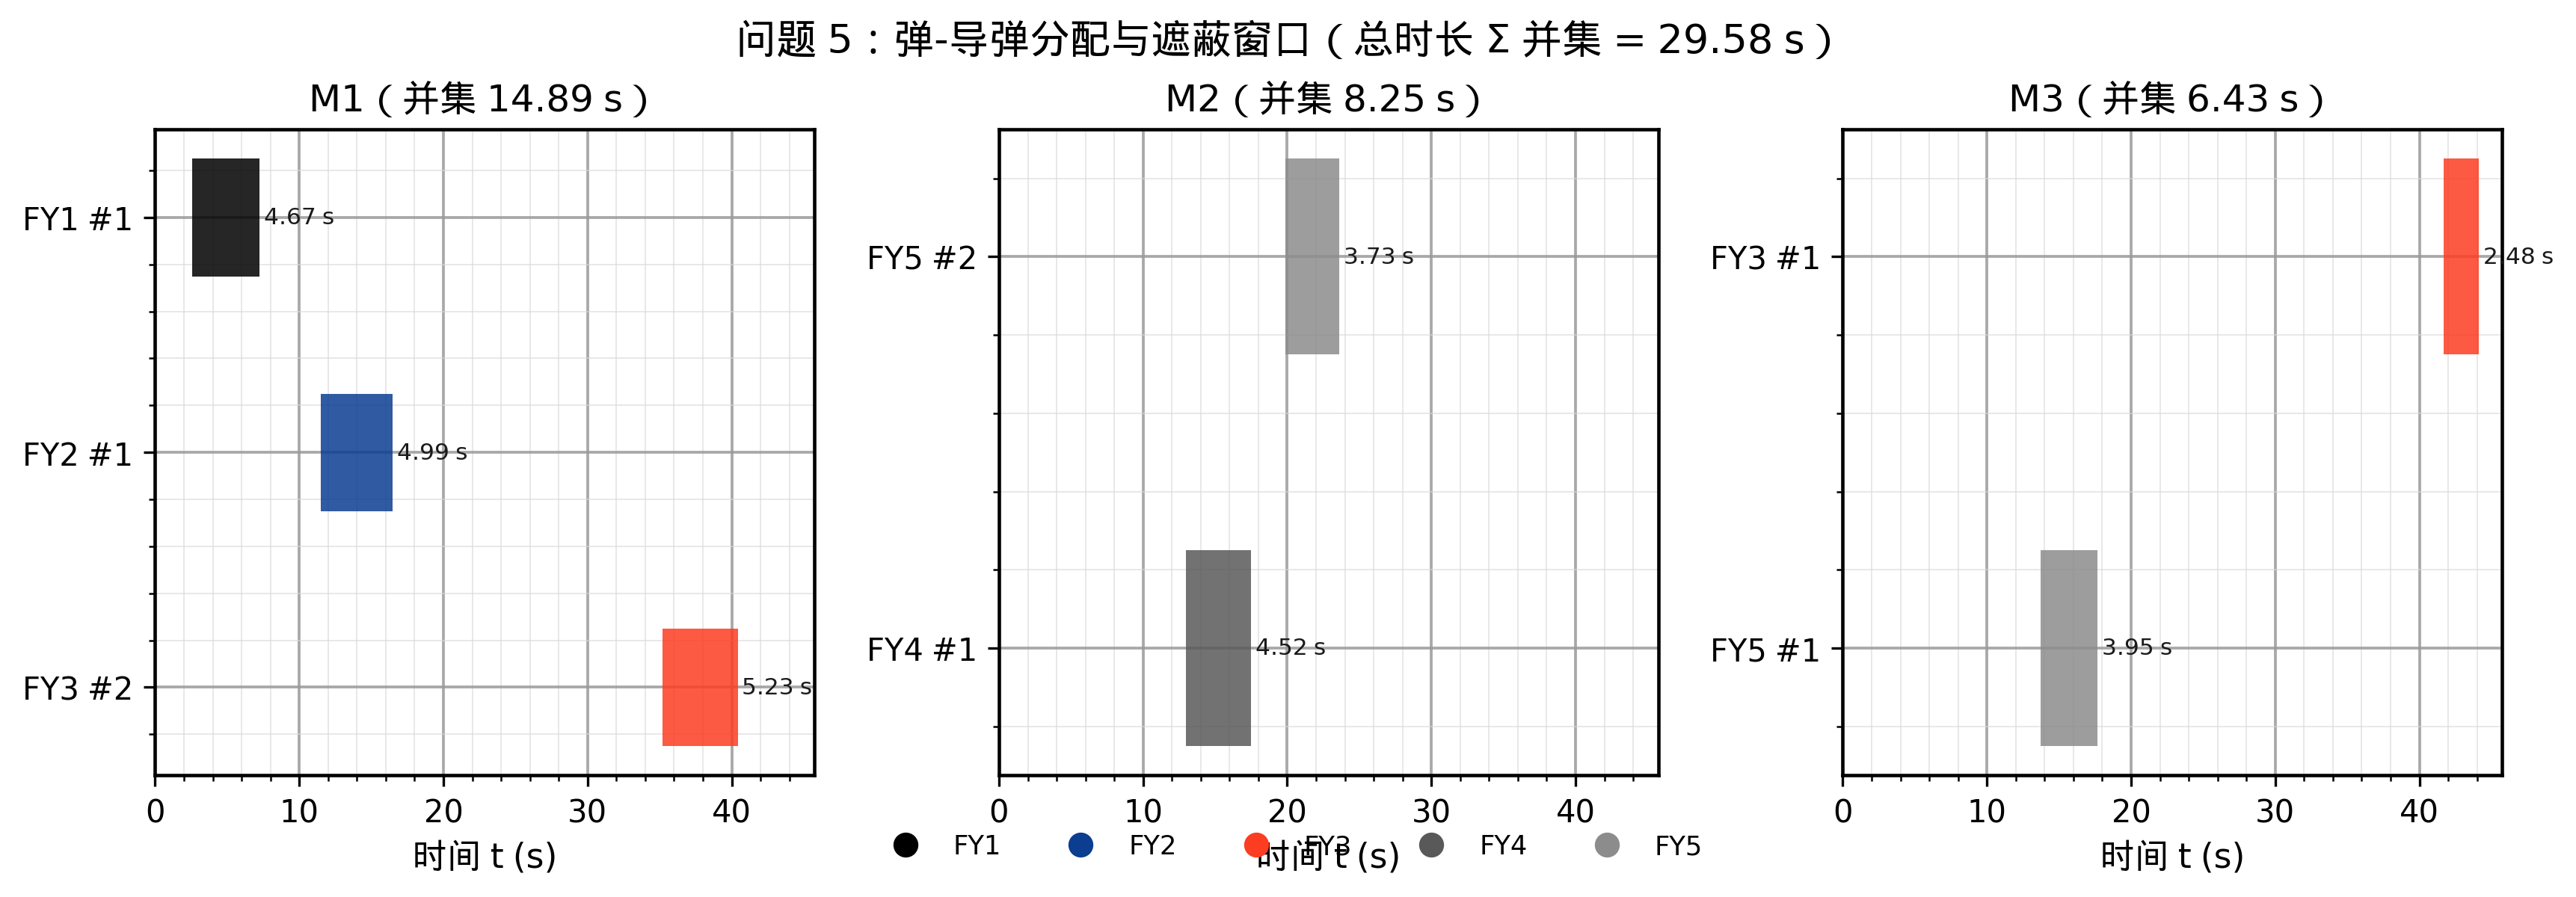
\includegraphics[width=\textwidth]{images/fig03_q5_assignment.png}
\caption{问题五弹—导弹分配与各弹遮蔽窗口（三面板共享时间轴，同一无人机颜色一致，条形末端标注时长）}
\label{fig:q5assign}
\end{minipage}
\end{figure}

%% ==================== 7. 模型的分析与检验 ====================
\section{模型的分析与检验}

\subsection{灵敏度分析}

对六类关键参数施加扰动，重评估各问题最优策略下的遮蔽时长，结果如表~\ref{tab:sensitivity}
所示（表中数值为固定策略在扰动物理下的重评估结果，不含重优化）。

\begin{table}[H]
\centering
\caption{参数扰动下各问题最优策略的有效遮蔽时长（单位 s）}
\label{tab:sensitivity}
\begin{tabular}{lcccccc}
\toprule
\textbf{参数} & \textbf{扰动} & Q2 & Q3 & Q4 & Q5 & 变化特征 \\
\midrule
导弹速度 & $-10\%$ & $4.85$ & $7.65$ & $15.18$ & $27.54$ & 敏感 \\
         & $+10\%$ & $4.17$ & $5.49$ & $12.77$ & $21.72$ & \\
云团下沉速度 & $-10\%$ & $4.73$ & $7.26$ & $16.21$ & $30.80$ & 中度 \\
             & $+10\%$ & $4.40$ & $7.18$ & $14.51$ & $27.68$ & \\
云团有效半径 & $-10\%$ & $4.15$ & $6.33$ & $13.82$ & $26.51$ & 敏感 \\
             & $+10\%$ & $5.01$ & $7.59$ & $16.59$ & $32.40$ & \\
云团有效时长 & $-10\%$ & $4.61$ & $7.26$ & $15.35$ & $29.58$ & 不敏感 \\
             & $+10\%$ & $4.61$ & $7.26$ & $15.35$ & $29.58$ & \\
重力加速度 & $-5\%$ & $4.40$ & $4.16$ & $6.13$ & $13.75$ & 策略未重优化 \\
            & $+5\%$ & $4.60$ & $4.45$ & $6.02$ & $16.16$ & 时降幅较大 \\
目标参考点高度 & $z=5$ m & $4.67$ & $7.26$ & $14.84$ & $29.80$ & 稳健 \\
              & $z=10$ m & $4.73$ & $7.26$ & $13.60$ & $28.98$ & \\
\bottomrule
\end{tabular}
\end{table}

灵敏度分析给出三点结论。第一，云团有效时长在 $18\sim22$ s 内变化对结果几乎没有影响，
说明各问题的遮蔽窗口宽度由视线几何扫掠决定，而非受 $20$ s 上限约束，模型中该参数取值
不构成瓶颈。第二，导弹速度与云团有效半径是最敏感的参数：导弹速度加快 $10\%$ 时视线扫掠
加快、遮蔽窗口压缩，问题五总时长下降约 $27\%$；有效半径缩小 $10\%$ 时遮蔽带收窄，总时长
下降约 $10\%$。对单弹问题在扰动物理下重优化，可达最优时长随导弹速度与下沉速度的变化约
为 $\pm4.5\%\sim\pm6.8\%$，随有效半径的变化约为 $\pm8.5\%\sim\pm10\%$，均未出现结论
方向性反转。第三，真目标参考点高度在 $0\sim10$ m 内变化时，问题二时长仅变化约 $3\%$，
说明"以 $(0,200,0)$ 为参考点"的建模选择是稳健的；重力加速度的固定策略重评估降幅较大，
但重优化后单弹最优仅变化约 $4.5\%$，属"策略未随物理重排"的预期现象，而非模型失效。
这些结论对实战运用有直接意义：导弹速度与云团有效半径是最需要谨慎核对的输入参数——
若来袭导弹速度被低估 $10\%$，按名义参数设计的策略会损失约两成遮蔽时长，因此在任务规划
时应留出速度余量或采用保守的投放窗口；相比之下，$20$ s 有效时长参数的偏差几乎不影响
方案，不必为其精确性耗费过多精力。目标参考点高度的稳健性则说明，把真目标近似为参考点
的建模方式在 $0\sim10$ m 的高度范围内是可信的。

综上，模型对关键参数扰动总体稳健。

\begin{figure}[H]
\centering
\begin{minipage}[t]{0.86\textwidth}
\centering
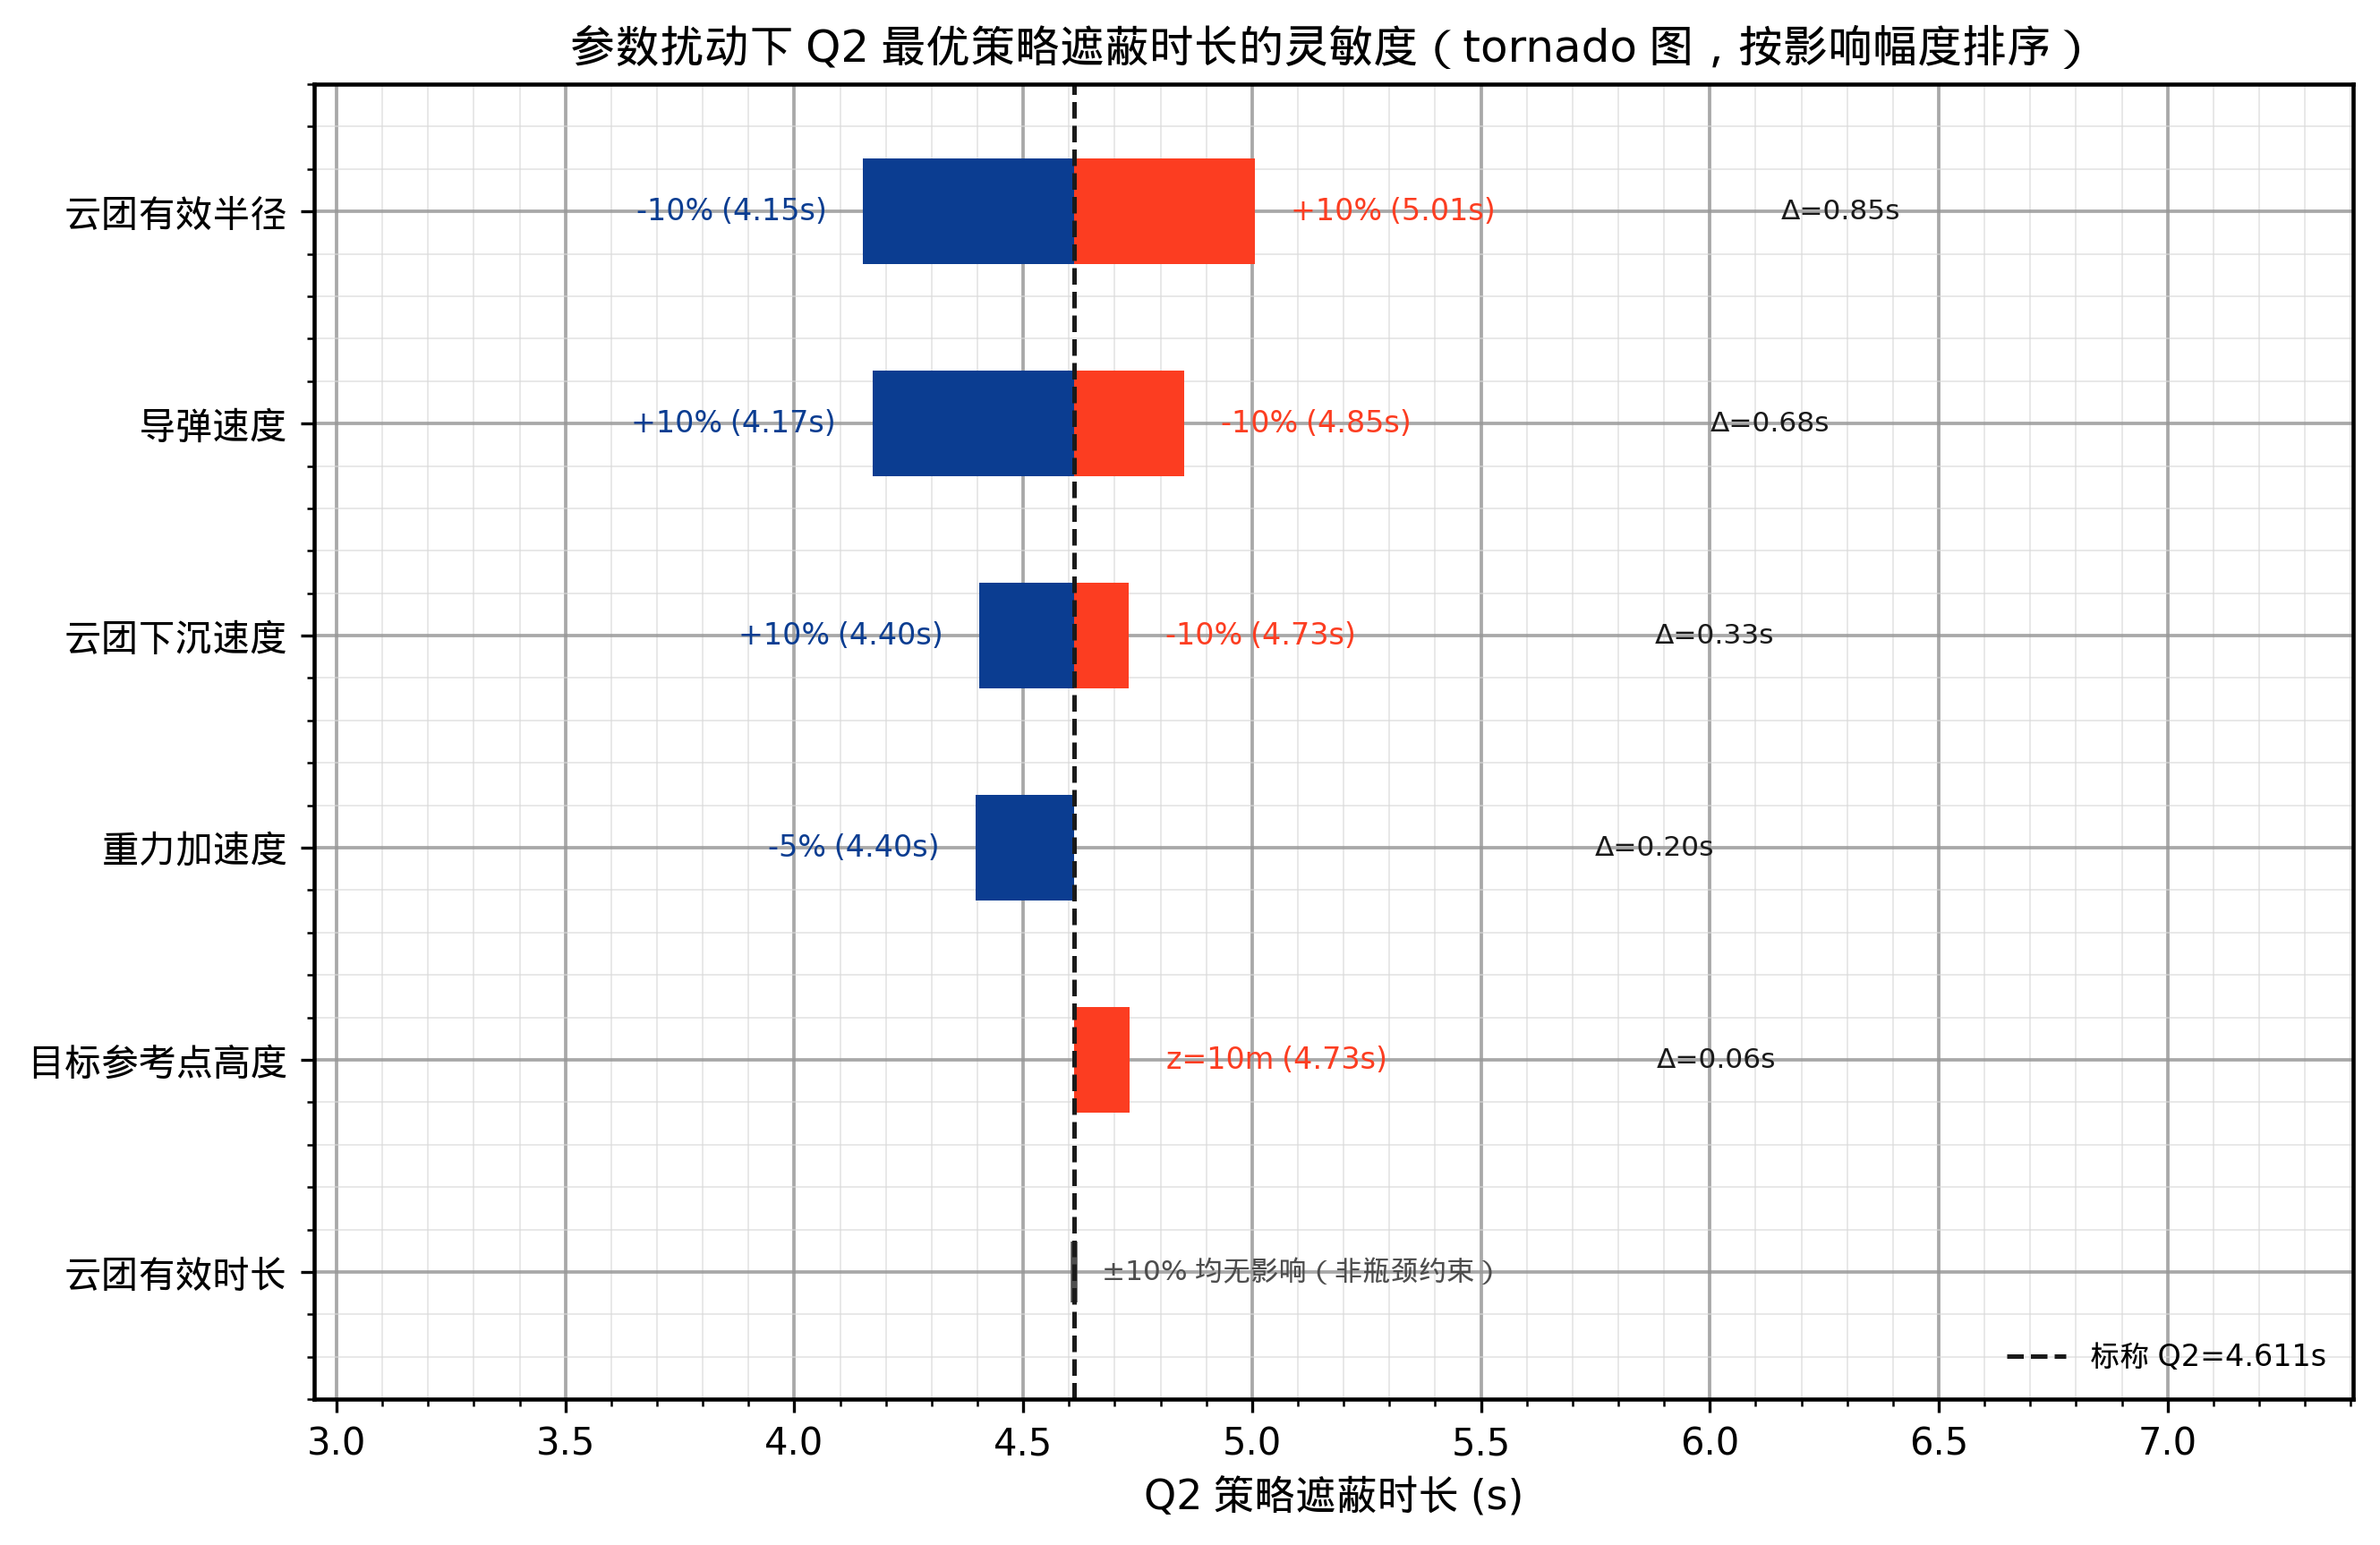
\includegraphics[width=\textwidth]{images/fig04_sensitivity.png}
\caption{参数扰动下问题二最优策略遮蔽时长的灵敏度（tornado 图，按影响幅度从大到小
排序，每行右侧标注影响幅度 $\Delta$；云团有效时长一行显示±10\%均无影响，说明该参数在当前解附近不构成瓶颈约束）}
\label{fig:sens}
\end{minipage}
\end{figure}

\subsection{模型验证}

全部求解代码均配有独立验证脚本，通过三项门控后结果方可进入论文（
AutoMCM-Pro 强制自证协议）。验证按优化模型与动力学模型两类检查清单执行：问题二至
问题五的最优解先做可行性检查，确认航向、速度、投放时刻与起爆延迟全部落在取值域内，
同机相邻投放间隔不小于 $1$ s；再做交叉验证，问题二与问题三用全定义域粗网格枚举作为
独立方法复核，网格最优时长不高于精化结果，问题四、五由结果文件反解参数重算的并集与
缓存一致。扰动测试对最优解各变量施加 $\pm0.1\%$ 随机扰动，均未产生更优遮蔽时长，
确认解位于局部最优平台。运动学自证逐项核对物理关系：起爆点与"投放点 + 无人机初速 +
重力"的解析公式误差小于 $10^{-6}$ m，云团中心每秒下沉恰好 $3$ m，三枚导弹均以
$300$ m/s 直线飞向假目标。单调性检查验证了资源增加不劣化结果的预期——问题三并集
时长不小于问题二单弹最优，问题四不小于问题二，问题五不小于问题四。最后检查并集测度
与弹—导弹分配：手工合并遮蔽区间与程序并集测度一致（误差 $<0.02$ s），问题五每枚弹
对其指派导弹的遮蔽时长均大于 $0$，分导弹并集之和与总时长一致。

问题一给定策略的正演结果亦用更细的时间步长（$0.005$ s）独立重算，与主结果 $1.410$ s
完全一致，确认数值实现无网格依赖性。全部验证检查共 $33$ 项（模型一 $9$ 项、模型二 $9$ 项、
模型三 $9$ 项、灵敏度 $5$ 项、数据预处理 $1$ 项），全部通过。

五个问题的有效遮蔽时长汇总于表~\ref{tab:summary}。从问题一到问题五，随着可调度资源
（弹数、无人机数、可干扰导弹数）的逐级放大，总遮蔽时长由 $1.410$ s 增长到 $29.580$ s，
增幅超过二十倍。这一增长并非线性：问题三相对问题二仅增加 $2.65$ s，而问题四相对问题三
翻倍有余，问题五又在此基础上接近翻倍——原因是多机协同打破了单机共用航向的约束，多导弹
并行的分配结构又让不同方向的来袭威胁能够同时被覆盖。

数值精度方面，遮蔽区间端点由二分法收敛到 $10$ m 边界的精确时刻，区间长度对时间步长
不敏感；优化结果对 $\pm0.1\%$ 参数扰动保持稳定，确认各最优解位于局部最优平台上。此外，
结果文件（result1/2/3.xlsx）的填写由程序直接回写，并经过独立脚本核对列值范围与有限性，
杜绝了手工抄录引入的笔误。

各阶段验证检查项按模型类型汇总于表~\ref{tab:verifysum}。所有检查项均通过后，对应阶段
才被批准进入下一环节，验证报告原文保留在流水线状态目录中备查。

\begin{table}[H]
\centering
\caption{各阶段验证检查项汇总（全部通过）}
\label{tab:verifysum}
% 原先用 lcl 定宽列，"覆盖内容"这一列文字较长时会把整张表撑出页面右边界
% （复核编译日志发现 414.75897pt Overfull \hbox，约 5.7 英寸溢出，肉眼就能
% 看到表格右侧出边）——改用 array 宏包的 p{} 定宽列强制换行，不再溢出。
\small
\begin{tabular}{>{\raggedright\arraybackslash}p{3.1cm}>{\raggedright\arraybackslash}p{3.6cm}>{\raggedright\arraybackslash}p{7.2cm}}
\toprule
\textbf{验证脚本} & \textbf{检查项} & \textbf{覆盖内容} \\
\midrule
\texttt{verify\_\allowbreak problem1\_\allowbreak geometry.py} & V-OPT-1$\sim$3, V-ODE-1$\sim$4, V-REG-1 & 可行性、交叉验证、扰动、弹道、云团、导弹运动学、遮蔽边界、Q1 回归 \\
\texttt{verify\_\allowbreak problem2\_\allowbreak schedule.py} & V-OPT-1$\sim$3, V-ODE-1$\sim$3, V-CONS-1$\sim$2, V-XLSX & 三弹时序可行域、并集逻辑、单调性、result1 填写 \\
\texttt{verify\_\allowbreak problem3\_\allowbreak multiuav.py} & V-OPT-1$\sim$3, V-ODE-1$\sim$3, V-CONS-1$\sim$2, V-XLSX & 多机可行域、分配正确性、单调性、result2/3 填写 \\
\texttt{verify\_\allowbreak sensitivity.py} & V-SEN-1$\sim$5 & 单调性、参考点稳健性、数值稳定、方向合理 \\
\bottomrule
\end{tabular}
\end{table}

\begin{table}[H]
\centering
\caption{五个问题有效遮蔽时长汇总}
\label{tab:summary}
\begin{tabular}{lccc}
\toprule
\textbf{问题} & \textbf{资源规模} & \textbf{有效遮蔽时长} & \textbf{相对上一问提升} \\
\midrule
问题一 & FY1 单弹，策略给定 & $1.410$ s & --- \\
问题二 & FY1 单弹，策略优化 & $4.611$ s & $+227\%$ \\
问题三 & FY1 三弹 & $7.263$ s & $+58\%$ \\
问题四 & FY1--FY3 各一弹 & $15.354$ s & $+111\%$ \\
问题五 & 五机 $\times$ 至多三弹 $\times$ 三导弹 & $29.580$ s & $+93\%$ \\
\bottomrule
\end{tabular}
\end{table}

%% ==================== 8. 模型的评价、改进与推广 ====================
\section{模型的评价、改进与推广}

\subsection{模型优点}

本模型在机理与算法两个层面各有可取之处。从求解效率看，物理启发多起点使优化器无需
在零值平原上盲目搜索：问题二约 $370$ 个起点、问题三约 $1080$ 个起点，配合两级坐标轮换
精化，单弹与三弹问题的求解均在一分钟量级完成；问题四的联合精化与问题五的分阶段框架
（15 组单弹优化 + 贪心分配 + 局部精化）在十分钟量级完成全部五问的求解。相比随机初始化
的全局搜索，这一策略把无效求值减少了两个数量级以上，同时保持了结果的可复现性。机理层面，五问共用同一套三维视线遮挡几何模型，
把"遮蔽"这一物理概念精确翻译为云团中心到视线线段距离不超过 $10$ m 的数学判据，并用
点—线段距离排除了云团位于导弹后方或目标后方时的误判；遮蔽时间按区间并集测度计取，
天然支持题目"遮蔽可不连续"的要求。算法层面，针对遮蔽时长可行域极窄、随机初始化难以
触及的特点，设计了物理启发多起点与坐标轮换精化相结合的求解策略，问题二、三的粗网格
交叉验证均确认精化结果不低于独立枚举；问题五的分阶段框架把数十维的联合优化分解为
单弹优化、贪心分配与局部精化三个可解释的环节，兼顾了求解效率与策略的可读性。

\subsection{模型局限性}

模型的主要局限来自三条简化假设。其一，遮蔽判据以真目标参考点代替整个圆柱体，未显式
考虑 $7$ m 半径柱体轮廓对判据的影响，不过灵敏度分析表明参考点高度在 $0\sim10$ m 内变化
对结果影响很小。其二，弹道忽略空气阻力与风场，烟幕云团按均匀球体处理，与真实烟幕的
扩散过程存在偏差；若存在高空风，云团漂移会改变遮蔽窗口的位置与长度。其三，问题五的
贪心分配是启发式算法，虽然通过按机方向重配与局部精化做了补偿，但不保证全局最优。

\subsection{改进方向与推广}

灵敏度分析还提示了一个值得注意的局限：重力加速度的固定策略重评估显示，当物理参数
偏离名义值时，未重优化的策略性能会明显回落（如问题五在 $g$ 减小 $5\%$ 时降幅过半）。
这说明本文给出的是"名义参数下的最优策略"，而非对参数不确定性鲁棒的自适应策略；在实战中
若存在参数漂移，需要结合实时测量对投放参数做在线修正。

改进可以从三个方向展开：一是把遮蔽判据升级为圆柱轮廓的完整遮挡判定，并引入风场与
烟幕扩散模型，使遮蔽几何更贴近物理实际；二是用精确算法（如混合整数规划对投放时序
离散化）求解问题五的分配子问题，给出最优性下界；三是引入多目标框架，在遮蔽时长、
弹药消耗与无人机航程之间做权衡，并考虑导弹机动（蛇形机动、多弹齐射）下的鲁棒策略。
本文的几何运动学正演模型与分阶段优化框架同样适用于烟幕遮蔽之外的其他"投放—拦截"
类问题，如诱饵弹投放、干扰机航迹规划与多平台协同防护，具备较好的可推广性。
%% ==================== 9. 参考文献 ====================
\section*{参考文献}
\addcontentsline{toc}{section}{参考文献}

\begin{thebibliography}{99}

\bibitem{Xiang2025}
Xiang C, Peng L. Effect of smoke screen interference on the hit rate of infrared imaging guidance[C]. Tenth Symposium on Novel Optoelectronic Detection Technology and Applications, 2025. DOI: 10.1117/12.3055707.

\bibitem{Ganagi1999}
Ganagi M, Singh S. Approximate closed-form solution for projectile trajectory and its applications to lead angle computations[J]. Defence Science Journal, 1999, 49(4). DOI: 10.14429/dsj.49.3827.

\bibitem{Zhang2023}
Zhang H, Zhu Y, Wang X, Li J. Research on evaluation method of anti-infrared smoke screen interference performance[C]. Advanced Fiber Laser Conference (AFL2022), 2023. DOI: 10.1117/12.2667063.

\bibitem{Storn1997}
Storn R, Price K. Differential evolution -- a simple and efficient heuristic for global optimization over continuous spaces[J]. Journal of Global Optimization, 1997, 11(4): 341-359. DOI: 10.1023/A:1008202821328.

\bibitem{Aggarwal2020}
Aggarwal S, Kumar N. Path planning techniques for unmanned aerial vehicles: A review, solutions, and challenges[J]. Computer Communications, 2020, 149: 270-295. DOI: 10.1016/j.comcom.2019.10.014.

\bibitem{Zheng2026}
Zheng Y, Liang X, Zhong L, et al. Distributionally robust integrated "decision--control" task assignment for multiple unmanned aerial systems in emergency response under stochastic disturbances[J]. Mathematics, 2026, 14(17): 3044. DOI: 10.3390/math14173044.

\end{thebibliography}

%% ==================== 附录 ====================
\appendix
\section{核心代码}

本文全部求解代码位于工作区的 \texttt{src/models/} 与 \texttt{src/verifications/}
目录。按 AutoMCM-SOP 附录节选规则，每个模型文件
仅收录体现核心求解逻辑的函数节选（用 \texttt{firstline}/\texttt{lastline} 直接从真实
源文件截取，与源文件自动保持同步）；验证脚本不收入附录，其结构化验证报告已在正文
第 7.2 节汇总。

\subsection{共享几何运动学模型（\texttt{geometry\_core.py}）}

遮蔽判据与遮蔽区间精化核心（完整文件另 231 行，含弹道/云团/导弹运动学）：
\lstinputlisting[style=pythonstyle, firstline=114, lastline=150,
  caption={遮蔽判据与区间精化核心}]{../src/models/geometry_core.py}

\subsection{问题一、二求解（\texttt{problem1\_geometry.py}）}

单机单弹投放策略优化核心（完整文件另 357 行，含问题一正演计算与绘图）：
\lstinputlisting[style=pythonstyle, firstline=147, lastline=187,
  caption={问题二优化核心：物理启发多起点 + 坐标轮换精化}]{../src/models/problem1_geometry.py}

\subsection{问题三求解（\texttt{problem2\_schedule.py}）}

单机三弹投放时序优化核心（完整文件另 278 行，含排序参数化与结果导出）：
\lstinputlisting[style=pythonstyle, firstline=140, lastline=192,
  caption={问题三优化核心：三弹并集遮蔽最大化}]{../src/models/problem2_schedule.py}

\subsection{问题四、五求解（\texttt{problem3\_multiuav.py}）}

多机协同联合优化核心（完整文件另 896 行，含问题五的贪心分配与分阶段框架）：
\lstinputlisting[style=pythonstyle, firstline=285, lastline=356,
  caption={问题四求解核心：多起点联合精化}]{../src/models/problem3_multiuav.py}

\subsection{灵敏度分析（\texttt{sensitivity.py}）}

参数扰动下的单弹重优化核心（完整文件另 309 行，含六类参数扰动表与绘图）：
\lstinputlisting[style=pythonstyle, firstline=116, lastline=147,
  caption={灵敏度重优化核心}]{../src/models/sensitivity.py}

\end{document}
